\chapter{Review of PDF determination}
\label{ch:pdfdet}
Understanding the functional structure of parton distributions is a complex task that has been subject to a number of approaches over the years. As nonperturbative quantities describing the behaviour of QCD bound states, in principle they may be subject to analysis using Lattice QCD methods. While a great deal of effort and progress has been made in understanding PDFs through nonperturbative methods~\cite{Dolgov:2000ca,Horsley:2004uq,Gockeler:2004wp,Schroers:2005rm}, results remain short of providing distributions for practical application at hadron colliders.

The majority of PDF analyses are therefore performed analogously to the determination of many other QCD parameters; via a fit to appropriate experimental data. The fundamental difficulty in PDF fits being that they are determinations of \emph{functions} rather than single parameters and therefore one must attempt to find some optimum solution in an (in principle) infinite-dimensional functional parameter space. This is of course complicated by having only a finite set of experimental data points upon which to perform a fit. Moreover as the applications involving PDFs have become more precise, a detailed understanding of the uncertainties in the determination of PDFs has become vital. The problem of PDF fitting is therefore one of finding a reliable estimator for a probability distribution in a space of functions.

The complexity of the task, along with the inherent ambiguities in the QCD treatment of data, led to the emergence of several competing methodologies and determinations. Today there are a diverse array of fitting groups producing sets of parton distribution functions, the most important of which being the ABM~\cite{Alekhin:2013nda,Alekhin:2012ig} (formerly ABKM~\cite{Alekhin:2009ni}), CTEQ/CJ~\cite{Gao:2013xoa,Lai:2010vv,Nadolsky:2008zw,Owens:2012bv}, JR/GJR~\cite{JimenezDelgado:2008hf,Gluck:2007ck}, HERAPDF~\cite{Aaron:2009aa,::2014uva}, MSTW~\cite{Martin:2009iq,Martin:2012da} (formerly MRST~\cite{Martin:1998sq,Martin:2001es,Martin:2002dr,Martin:2004dh}) and NNPDF~\cite{Ball:2012cx,Ball:2011gg,Ball:2011uy,Ball:2011mu,Ball:2010de,Ball:2008by} groups. Typically PDF sets are provided for a variety of theory input parameters such as perturbative order, and value of the strong coupling. All modern PDF sets now include a quantitative assessment of their associated uncertainties. In this chapter we shall review the ingredients and methods utilised in a modern PDF determination, primarily focusing on the methodology of the three global PDF fits recommended for LHC phenomenology by the PDF4LHC working group~\cite{Botje:2011sn}, namely the procedures of the CTEQ, MSTW and NNPDF collaborations.

These three groups produce PDF sets determined from a fit to a wide range of experimental data, including DIS, Drell-Yan and inclusive jet cross sections. The CTEQ and MSTW determinations follow a similar fitting procedure and method of uncertainty estimation, with the NNPDF group taking a rather different approach to both. We will now describe the basic fitting procedure of these groups, with an eye to detailing areas where the groups have different solutions.

\section{Experimental data on parton distributions before the LHC}
The most important ingredient in the determination of parton distributions is naturally the selection of the dataset from which to extract PDF constraints. The first step in performing a PDF fit is therefore to identify which datasets are most sensitive to input parton distributions, and offer precise and reliable data. As PDF determinations to date have relied only upon fixed-order perturbation theory, the dataset chosen should probe sufficiently inclusive observables which are therefore relatively insensitive to resummation effects. In general PDF fitting collaborations also require data to be taken at a sufficiently high scale that leading-twist factorisation remains reliable, although there are some exceptions which we shall discuss later in the section. Here we shall briefly discuss some of the most important processes in terms of PDF sensitivity, and review some of the most relevant experimental measurements. For this section we shall restrict ourselves to data available before the start of LHC operation in order to provide a background for the methodological developments made in the light of LHC data. 

\subsubsection{Fixed-Target and collider DIS}
Deep inelastic scattering data provides the backbone for much of a PDF analysis, and data is available from a wide array of sources. Precise electron-proton scattering data from HERA provides the cleanest probe of proton structure function data, while high-luminosity fixed-target experiments can provide important constraints, at the expense of potentially having to deal with additional data corrections due to nuclear and higher-twist effects. As DIS is one of the best understood scattering processes in QCD, precise theoretical predictions are available up to 3-loop order in the zero-mass scheme~\cite{Vermaseren:2005qc,Moch:2008fj} and 2-loop order with full heavy quark masses intact~\cite{Buza:1997mg,Buza:1996xr,Blumlein:2006mh,Bierenbaum:2007qe,Bierenbaum:2007dm,Bierenbaum:2009zt,Blumlein:2014fqa}.

At leading order, neutral current DIS measurements from a proton target directly probe the quark sea distributions $q_i+\bar{q}_i$, with the relative power of each flavour contribution mediated via its coupling to $\gamma,Z$. Charged current, and $Z$-mediated neutral current data can provide some constraint upon PDF flavour separation via the $F^3$ structure function. 

In addition to proton structure function measurements, data obtained from scattering off deuterium targets can be important in constraining light quark flavour separation under the assumption of isospin symmetry. Data may be presented as direct measurements of $F_d$ structure functions or as the ratio $F_d/F_p$. A simultaneous fit to deuterium and proton data may therefore provide important constraints upon the $u-d$ and $u/d$ PDF combinations. Data determined via deuteron scattering are subject to nuclear corrections e.g. shadowing effects~\cite{Badelek:1994qg} which may be estimated as part of the theoretical treatment or neglected; the corrections to be considered part of the theory uncertainty.

Alongside the direct information on quark distributions, scaling violations present in structure function data provide constraints upon the gluon. While rather indirect, the wealth of DIS measurements available at a wide range of scales provides a great deal of information on the structure of the gluon distribution.

DIS data may be presented either as experimental cross sections, or separated into structure functions. Fixed target structure function data on $F_2$ from muon scattering is available for both proton and deuteron targets from the BCDMS~\cite{Benvenuti:1989rh,Benvenuti:1989fm}, NMC~\cite{Arneodo:1996qe,Arneodo:1996kd} and Fermilab E665~\cite{Adams:1996gu} experiments. Electron scattering $F_2$ data is also available from SLAC data on both proton and deuteron targets~\cite{Whitlow:1991uw}. The longitudinal structure function $F_L$ is measured in fixed target experiments also by SLAC~\cite{Whitlow:1990gk} , BCDMS~\cite{Benvenuti:1989rh} and NMC~\cite{Arneodo:1996qe}. 

In addition to the large datasets available from fixed target experiments, HERA data provides a clean probe of DIS properties, although with HERA data the separation of cross-sections into structure functions is typically not performed. Neutral current cross-section data is provided by ZEUS~\cite{Breitweg:1998dz,Chekanov:2001qu,Chekanov:2002ej,Chekanov:2003yv} and H1~\cite{Adloff:2000qk,Adloff:2000qj,Adloff:2003uh}. Charged-current DIS data is also provided by the HERA collaborations \cite{Chekanov:2003vw,Adloff:2003uh} along with information on the longitudinal structure function $F_L$~\cite{Andreev:2013vha,Chekanov:2009na}. Information on charm hadroproduction in DIS is available via $F_2^{\mathrm{charm}}$ measurements at HERA also~\cite{Adloff:1996xq,Adloff:2001zj,Aktas:2005iw,Aktas:2004az,Breitweg:1999ad,Chekanov:2003rb,Chekanov:2007ch}. This data provides particular constraint upon the gluon PDF, and has been an important testing ground for heavy quark flavour schemes. The clean $ep$ environment means that data is unaffected by nuclear or deuteron corrections, although low energy datapoints may still suffer from substantial higher-twist corrections. These corrections are typically kept under control by kinematic cuts on the affected points, however some groups (notably the ABM/CJ groups) include the affected data and attempt to model the corrections.

HERA measurements from the two collaborations have been examined as a combined analysis and dataset, so far resulting in two studies of direct interest to PDF determination; a combination of HERA-1 inclusive DIS data~\cite{aaron:2009wt}, and of charm production cross-sections~\cite{Abramowicz:1900rp}.

\begin{figure}[ht]
\centering
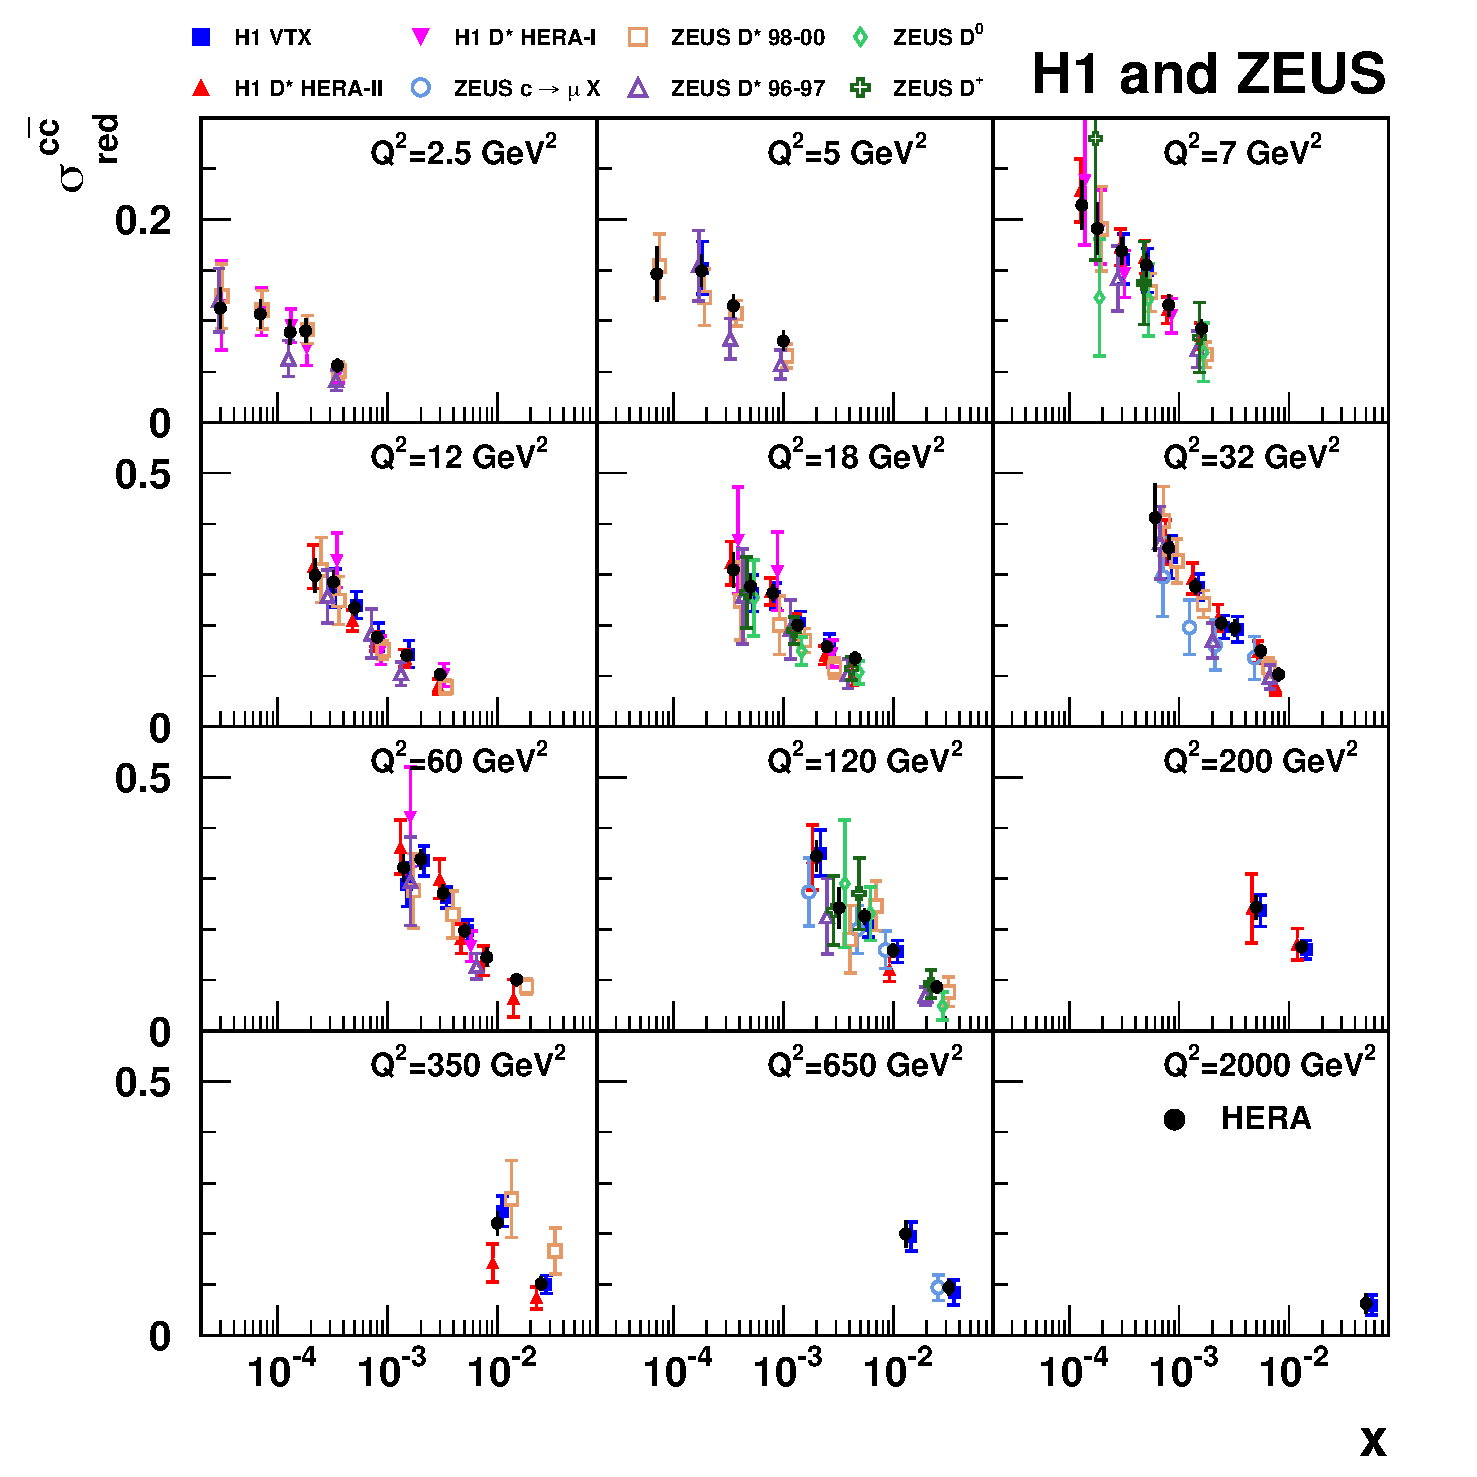
\includegraphics[width=0.8\textwidth]{3-PDFdet/figs/d12-172f3.pdf}
\caption[Combined reduced charm cross-section data from HERA]{Reduced charm cross-section data from the HERA combined measurement. Data from the measurements contained in the combination analysis is shown for comparison. Figure from \cite{Abramowicz:1900rp}.}
\label{fig:HERAF2c}
\end{figure}

The very large quantity of deep-inelastic scattering measurements performed at a variety of experimental facilities means that generally DIS data forms the backbone for PDF fits, providing a substantial proportion of the experimental data points used in a fit.

\subsubsection{Neutrino DIS}
There are a number of measurements available for the scattering of neutrino beams from heavy nuclear targets. For example the NuTeV~\cite{Tzanov:2005kr} and CHORUS~\cite{Onengut:2005kv} data on neutrino $F_2$ and $F_3$. Assuming an approximately isoscalar target, and neglecting CKM factors, the PDF dependence of the neutrino structure function data at leading order is given by~\cite{Forte:2013wc}
\begin{eqnarray}
	F_2^\nu(x) &=& x\left( u^+(x) + d^+(x) + 2s(x) + 2\bar{c}(x)\right), \\
	F_2^{\bar{\nu}}(x) &=& x\left( u^+(x) + d^+(x) + 2\bar{s}(x) + 2c(x)\right),
\end{eqnarray}
and for the $F_3$ structure function,
\ba
	F_3^\nu(x) &=& x\left( u^-(x) + d^-(x) + 2s - 2\bar{c}\right), \\
	F_3^{\bar{\nu}}(x) &=& x\left( u^-(x) + d^-(x) - 2\bar{s}(x) + 2c(x)\right).
\ea
A simultaneous fit of these data points therefore provides a good handle upon the valence quark distributions $q-\bar{q}$. These datasets are relatively precise; however they are subject to potentially large nuclear corrections which introduce an uncertainty that is poorly understood.

\begin{figure}[ht]
\centering
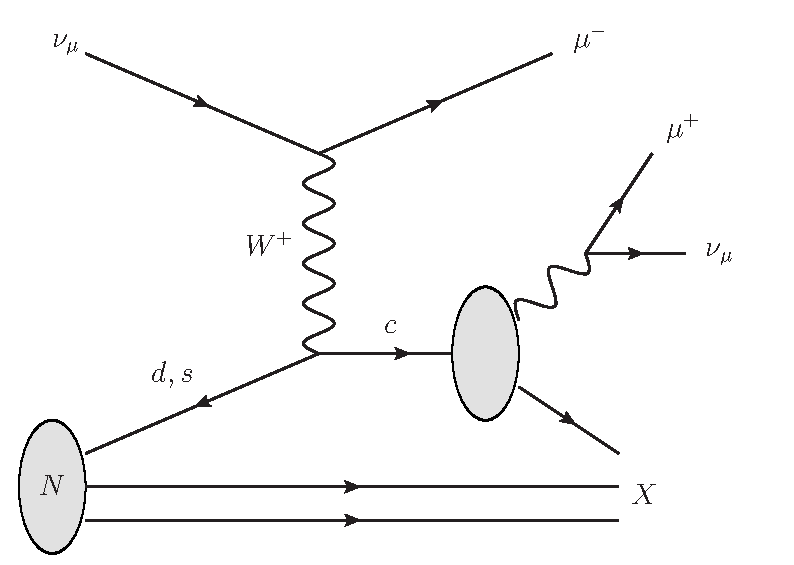
\includegraphics[width=0.5\textwidth]{3-PDFdet/figs/dimuon.pdf}
\caption[Leading order diagram for dimuon production in neutrino DIS]{Leading order diagram for dimuon production in neutrino DIS.}
\label{fig:dimuon}
\end{figure}

Neutrino DIS becomes particularly valuable for PDF determination when considering the semi-inclusive DIS dimuon production process $\nu N \to \mu\mu X$ illustrated in Figure \ref{fig:dimuon}. In this process the contribution from initial state strangeness is Cabbibo favoured, therefore providing a direct handle on the strange distribution whose contribution is ordinarily difficult to discern from total structure function measurements. Measurements of this process are therefore commonly used as a strangeness probe, and data has been provided by the NuTeV/CCFR collaborations~\cite{Goncharov:2001qe}.

\subsubsection{Fixed-target and collider Drell-Yan}
After DIS measurements, the production of electroweak vector bosons in hadronic collisions provides the next most important contribution to the constraint of parton densities, with precise predictions available at NNLO in QCD~\cite{Anastasiou:2003ds,Catani:2009sm,Catani:2010en}.  At leading order the neutral current Drell-Yan process is moderated by the PDF combination
		\be q(x_1)\bar{q}(x_2) +  \bar{q}(x_1)q(x_2),\ee
and provides a direct probe of various partonic combinations depending upon the experimental configuration. In the Drell-Yan process the relevant kinematic variables are the invariant mass of the lepton pair
\be M_{ll}^2 = (E_1 + E_2)^2 - (\mathbf{p}_1 + \mathbf{p}_2)^2,\ee
and the intermediate boson's rapidity, given in the detector frame by
\be y = \frac{1}{2}\log \frac{E+ p_L}{E-p_L},\ee
where $E$ is the detector frame energy of the intermediate boson, and $p_L$ its longitudinal momentum.  in terms of which the parton-$x$ is given by;
\be x_\pm = M_{ll} e^{\pm y} / \sqrt{s}, \ee
where $s$ is the centre-of-mass energy squared of the reaction and the $\pm$ denotes the parton direction with respect to the beam frame. High rapidity measurements therefore constrain PDFs at both high and low-$x$. 

Additionally the charged-current process $qq^\prime \to l^\pm \nu_l$ provides information on quark flavour separation in the initial state hadrons. While the rapidity of the lepton pair resulting from $Z/\gamma$ decay in neutral current Drell-Yan is experimentally straightforward to distinguish, the presence of a neutrino in the final state of $W$ production processes complicates the direct resolution of the $W$ rapidity. Therefore data is often presented in the pseudorapidity of the detected lepton,
\be \eta = -\log \tan \theta,\ee
defined in terms of the angle $\theta$ between the final state lepton and the beam axis. It can therefore be measured without knowledge of the particle mass and momentum. The pseudorapidity coincides with the standard rapidity in the case of massless particles where $E = |\mathbf{\bar{p}}|$.

Lepton asymmetries are another common form for experimental results in Drell-Yan, defined in terms of $W^{\pm}\to l^\pm\nu_l $ differential cross-sections $d\sigma_{l^\pm}/d\eta_l$ as
\be 
  A^l_W=\frac{d\sigma_{l^{+}}/d\eta_{l}-d\sigma_{l^{-}}/d\eta_{l}}
  {d\sigma_{l^{+}}/d\eta_{l}+d\sigma_{l^{-}}/d\eta_{l}}, 
\ee
such measurements also benefit from the cancellation of shared systematic uncertainties. Measurements of lepton pair production from proton beams incident upon heavy nuclear targets, such as the E605\cite{Moreno:1990sf} experiment determining dimuon production from a copper target are useful for the constraint of the light quark sea $q+\bar{q}$. These measurements are typically very precise but suffer from poorly determined nuclear corrections. Several approaches have been performed to study the extent of these corrections~\cite{deFlorian:2003qf,Hirai:2007sx,Kulagin:2007ju,Eskola:2009uj}, although the effects are typically small and may sometimes be discounted in comparison to experimental uncertainties~\cite{Ball:2009mk}. Contributions from initial state heavy quarks and strangeness are typically suppressed in these measurements due to the relatively low scales.

\begin{figure}[ht]
\centering
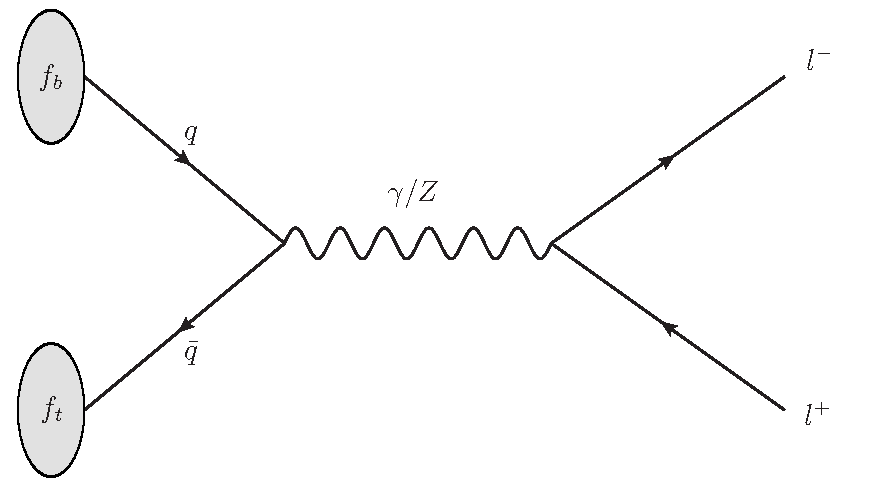
\includegraphics[width=0.45\textwidth]{3-PDFdet/figs/ncdy.pdf}
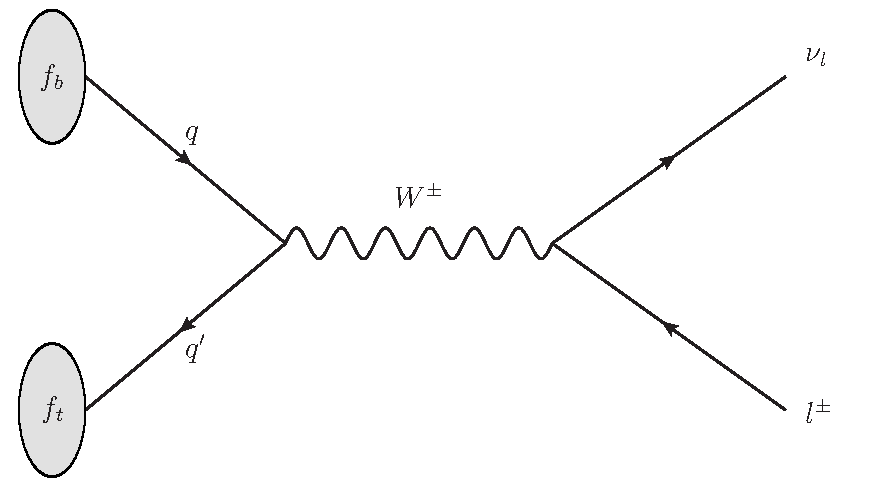
\includegraphics[width=0.45\textwidth]{3-PDFdet/figs/ccdy.pdf}
\caption[Leading order diagram for the Drell-Yan process]{Drell-Yan process at leading order, initiated by beam protons with PDF $f_b$ and target protons with PDF $f_t$. The neutral current process is shown on the left, and the charged current process on the right.}
\label{fig:ncdy}
\end{figure}

Fixed target experiments upon hydrogen or deuterium targets provide a relatively clean probe and the ratio of Drell-Yan cross sections in proton to deuteron targets can provide crucial information on the $u/d$ PDF combination. While relatively free of nuclear effects, deuteron data still suffers from poorly understood corrections, which have been the subject of extensive study\cite{Martin:2012da, Badelek:1994qg,Accardi:2011fa,Brady:2011hb}.
Experimental measurements from the Fermilab NuSea/E866 collaboration are commonly used, providing data from $pp$~\cite{Webb:2003bj} and $pd/pp$~\cite{Towell:2001nh} experiments.  

The theoretically cleanest environment to examine the Drell-Yan process is at high scales at a collider. Several measurements are available from the Tevatron collaborations which provide information free of nuclear or deuteron corrections. As a $p\bar{p}$ collider, neutral-current Drell-Yan at the Tevatron targets the quark valence contribution and asymmetry data provides information on the $u/d$ ratio. A measurement of the $Z$ rapidity distribution  is available from D0~\cite{Abazov:2007jy}, and several measurements are available for $W$ lepton asymmetries from both Tevatron collaborations \cite{Acosta:2005ud,Abazov:2007pm,Abazov:2008qv,Abe:1998rv}.

In order to obtain a handle on the contribution of initial state strange quarks to the Drell-Yan process it is once again necessary to examine less inclusive processes. Of particular interest are measurements of $W$ production in association with a charm jet, analogous to the usefulness of dimuon measurements in neutrino DIS where the strange contribution is favoured in terms of CKM elements. Measurements of this process were initially made at the Tevatron by both CDF~\cite{Aaltonen:2007dm} and D0~\cite{Abazov:2008qz}. More precise determinations can be obtained by normalisation with respect to the total $W+$ jets rate~\cite{Stirling:2012vh}. 

\subsubsection{Jet production data}
While DIS data provides constraints upon the gluon distribution via scaling violations and contribution to heavy quark and longitudinal structure functions, DIS and Drell-Yan data do not provide a substantial direct constraint upon gluon densities. The most constraining datasets for the gluon, particularly in the uncertain large-$x$ region, are those of jet production measurements. The large strong coupling of the gluon combined with a high gluon luminosity in the proton at high scales results in $gg$ initiated diagrams being the dominant sub channels for the production of inclusive jet and dijet events.

Cross-section calculations for inclusive jet and dijet data in hadron-hadron collisions are available at NLO in QCD~\cite{Ellis:1992en,Giele:1994gf,Nagy:2001fj,Nagy:2003tz}, however a great deal of progress has been made in the determination of the NNLO corrections~\cite{Currie:2013dwa,Glover:2001af,Glover:2001rd}, with the exact gluon-gluon sub channel calculation recently determined~\cite{Currie:2013dza}. For the full calculation however, only approximate NNLO results are available via threshold resummation techniques~\cite{deFlorian:2013qia,Kidonakis:2000gi,Kumar:2013hia}. Jet data may therefore only be included into an NNLO PDF fit through an approximate treatment if at all.

Jet data must be included via some clustering algorithm which takes a QCD final state and identifies suitable jet-like structures. Earlier measurements were performed with so-called cone algorithms, although these are potentially very sensitive to infrared and collinear effects. More recent experiments typically utilise sequential-combination algorithms such as the Cambridge-Aachen~\cite{Dokshitzer:1997in,Wobisch:1998wt}, $k_T$~\cite{Ellis:1993tq} or anti$-k_T$~\cite{Cacciari:2008gp} algorithms, often used as implemented in the efficient {\tt FastJet}~\cite{Cacciari:2011ma} package.

The CDF collaboration has published precise measurements of inclusive jet~\cite{Abulencia:2007ez,Aaltonen:2008eq} and dijet~\cite{Aaltonen:2008dn} cross sections. Data is also available from the D0 experiment, once again for inclusive~\cite{Abazov:2008ae} and dijet~\cite{Abazov:2010fr} quantities.
Figure \ref{fig:CDFkTJet} shows the results of an inclusive jet measurement at CDF using the $k_T$ clustering algorithm.
\begin{figure}[ht]
\centering
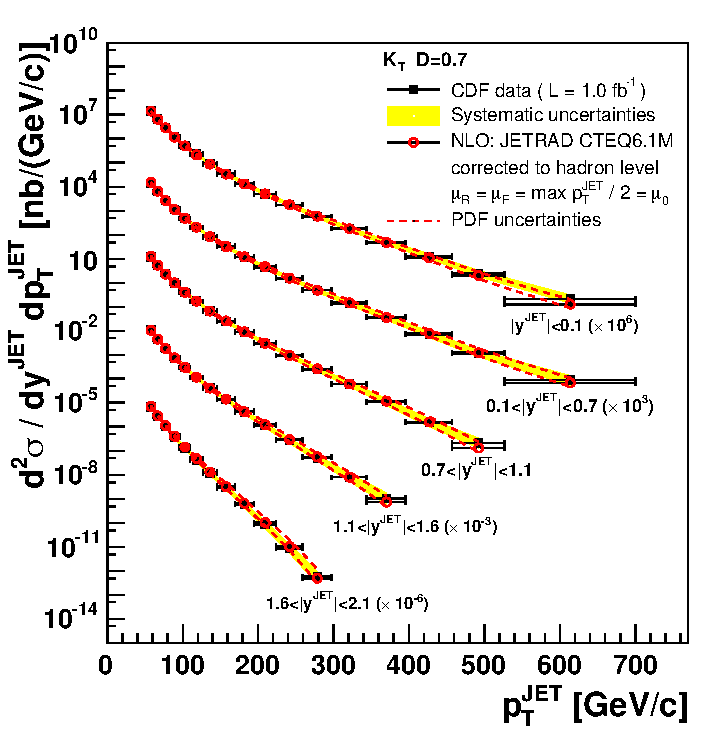
\includegraphics[width=0.6\textwidth]{3-PDFdet/figs/CrossSectionAll.pdf}
\caption[Inclusive Jet data from the CDF experiment]{Inclusive jet data from CDF using the $k_T$ jet clustering algorithm, compared to predictions from the CTEQ6.1M PDF set. Figure from~\cite{Abulencia:2007ez}. }
\label{fig:CDFkTJet}
\end{figure}

\subsubsection{Prompt photon measurements}
Complementary to the data on jet production, measurements of prompt photon processes $pp/p\bar{p} \to \gamma X$ can also provide an important handle on the gluon. The term \emph{prompt} photon refers the production of a photon in the hard scatter rather than in subsequent emissions. Prompt photons in the final state can originate either from Compton scattering processes $gq \to \gamma q$ or annihilation events $q\bar{q} \to \gamma g$, processes denoted \emph{direct} photon production. Alternatively prompt photons may be produced via the fragmentation of final state hadrons into photons via so-called fragmentation functions\cite{Bourhis:1997yu,Gluck:1992zx}. In $pp$ collisions the Compton scatter is typically the dominant process, particularly at higher scales where the fragmentation contribution is suppressed. For $p\bar{p}$ events the annihilation contribution becomes more important due to the enhanced $q\bar{q}$ PDF luminosity. Figure \ref{fig:jrpromptphoton} demonstrates the relative fraction of these contributions to the cross-section for a range of photon transverse energy $E_T$.
\begin{figure}[ht]
\centering
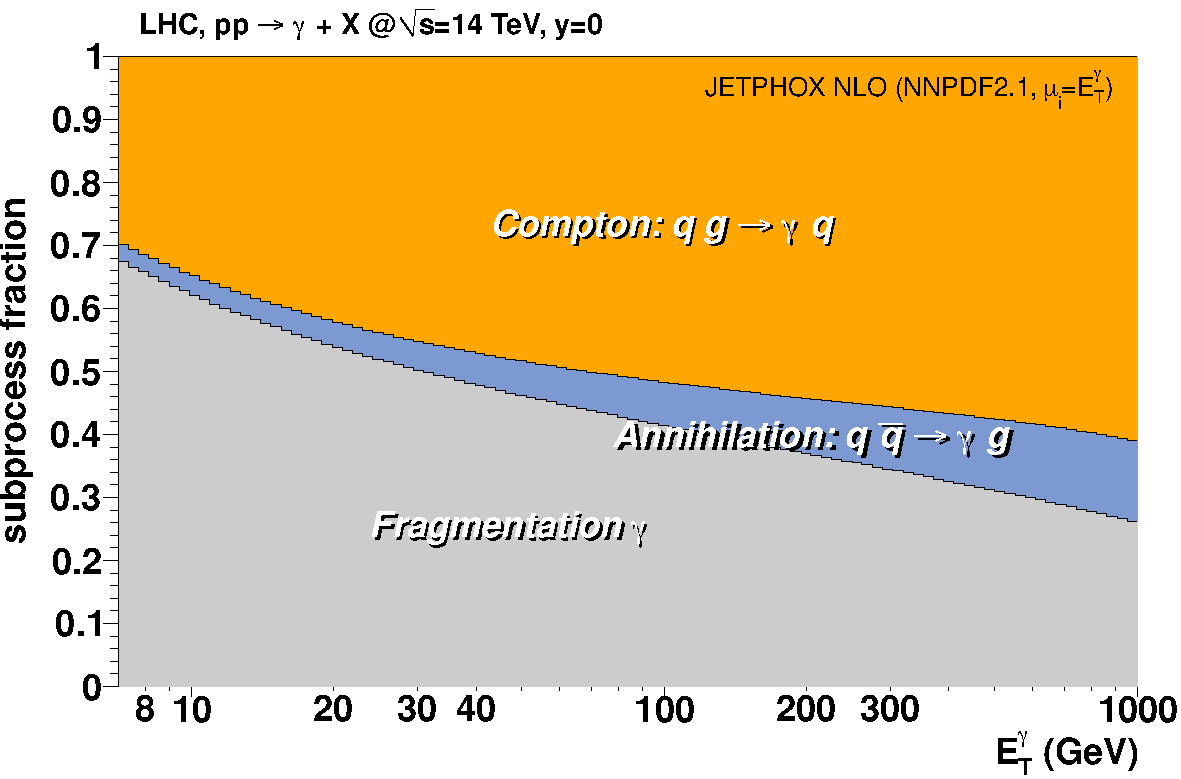
\includegraphics[width=0.48\textwidth]{3-PDFdet/figs/subproc_ppgamma_jetphox_lhc_inc_stack.pdf}
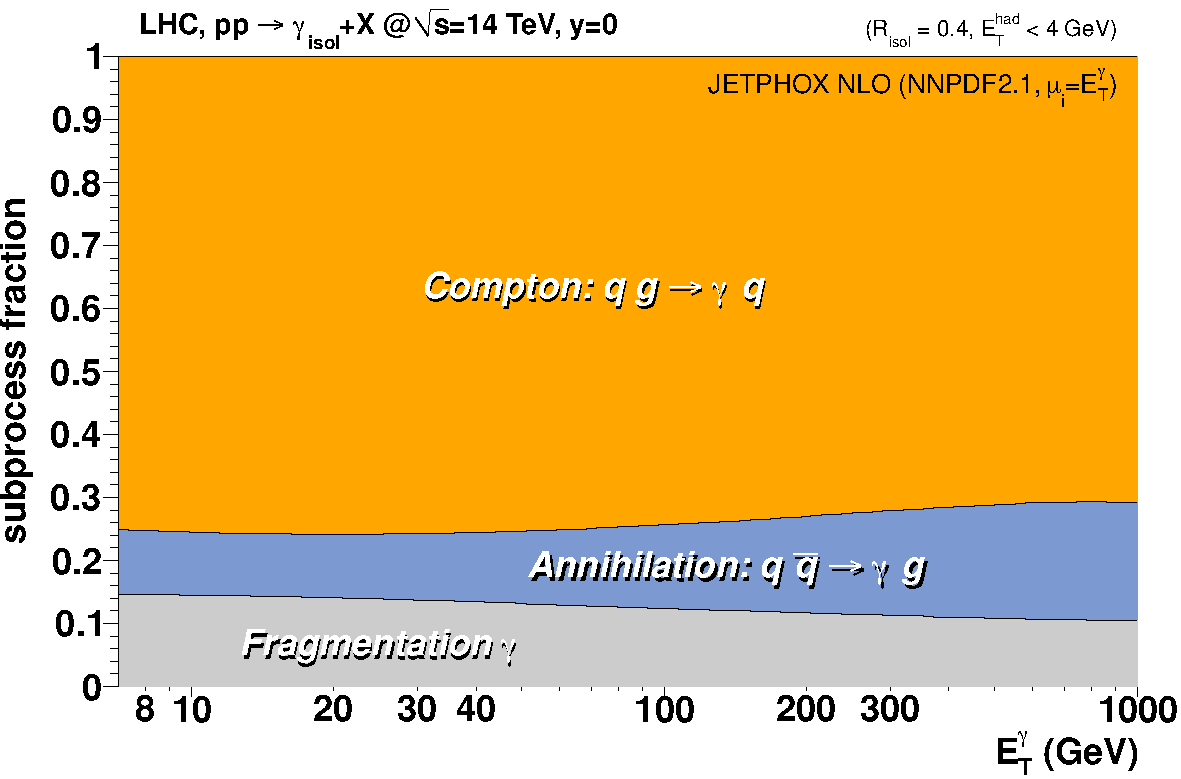
\includegraphics[width=0.48\textwidth]{3-PDFdet/figs/subproc_ppgamma_jetphox_lhc_is_stack.pdf}\\
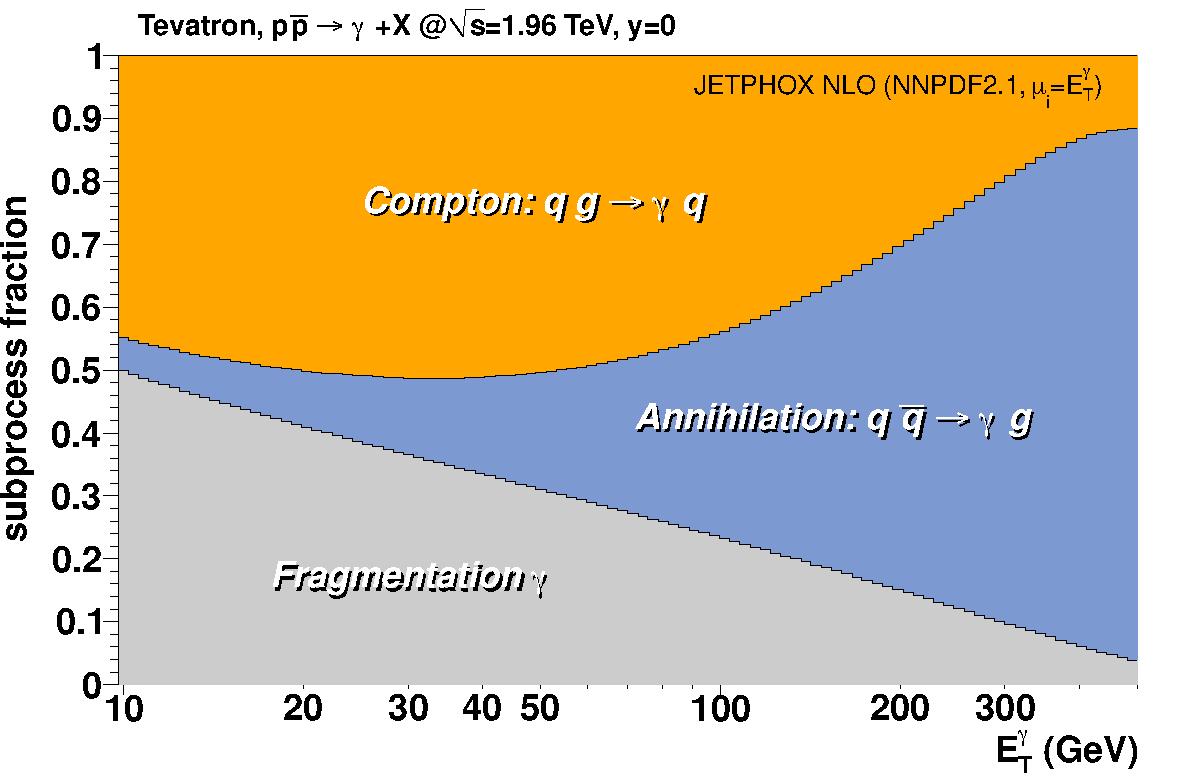
\includegraphics[width=0.48\textwidth]{3-PDFdet/figs/subproc_ppgamma_jetphox_tevatron_inc_stack.pdf}
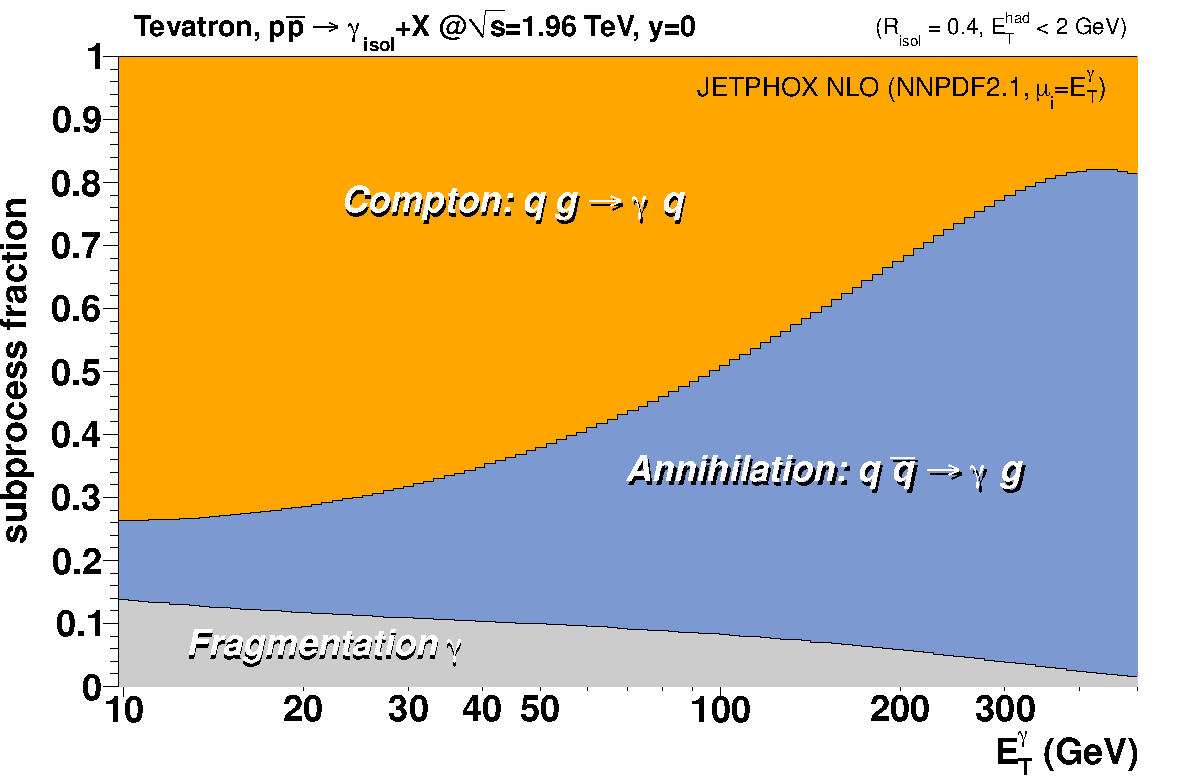
\includegraphics[width=0.48\textwidth]{3-PDFdet/figs/subproc_ppgamma_jetphox_tevatron_is_stack.pdf}
\caption[Relative contribution of partonic subprocesses to $pp/p\bar{p}\to \gamma X$]{Relative contribution of partonic subprocesses to $pp/p\bar{p}\to \gamma X$. Figures on the left refer to the inclusive case, and on the right to the observable after isolation cuts on the final state photon. Figure from~\cite{dEnterria:2012yj}. }
\label{fig:jrpromptphoton}
\end{figure}

For the purposes of PDF determination direct photon measurements which are free of the additional uncertainties introduced when performing calculations with photon fragmentation functions are the ideal measurement. While performing selection cuts to measure only the direct photon contribution is experimentally challenging, the relative contribution of fragmentation photons may be suppressed by making isolation cuts upon the final state photon. These cuts admit only photons with no hadronic material in close proximity. Smooth-cone cuts such as the Frixione isolation criterion~\cite{Frixione:1998jh} in principle can remove entirely the fragmentation contribution. However these cuts remain challenging to implement experimentally, with experimental data usually obtained with simpler isolation cuts which aim to suppress rather than eliminate fragmentation photons.

Theoretical predictions are available at NLO for the Compton process~\cite{Owens:1987qy,Aurenche:1988vi} and commonly used as implemented in the {\tt JETPHOX} program~\cite{Catani:2002ny,Aurenche:2006vj,Belghobsi:2009hx}. While inclusive data is challenging to include in a PDF determination due to contamination by fragmentation photons, results are available from a wide range of isolated photon measurements. Isolated data is available from  UA1/UA2 at the Sp$\bar{\mathrm{p}}$S~\cite{Albajar:1988im,Alitti:1992hn,Ansari:1988te}, PHENIX at RHIC~\cite{Adler:2006yt}, CDF~\cite{Aaltonen:2009ty,Abazov:2005wc,Abe:1994rra,Acosta:2002ya,Acosta:2004bg} and D0~\cite{Abachi:1996qz,Abazov:2001af,Abbott:1999kd}.

\subsubsection{Top quark pair production data}
The production of top-antitop pairs is potentially a process of great interest in the determination of PDFs, with calculations available up to NNLO for the total cross-section~\cite{Czakon:2013goa,Baernreuther:2012ws,Czakon:2012zr,Czakon:2012pz}. The impact of the total top pair production cross-section upon PDFs is quite sensitive to the kinematics of the collider, with Tevatron data probing directly the quark content of the proton, while data from colliders with higher centre of mass energies being dominated by the gluon-gluon channel. Precise data from the Tevatron is available in the form of a combined D0-CDF analysis~\cite{Aaltonen:2012ttbar}.

\subsubsection{Experimental cuts}
 A simple cut is typically performed on the hard scale $Q^2$ and for DIS the final state invariant mass $W^2$ to ensure the reliability of perturbative predictions. The MSTW2008 parton fit uses an initial scale for evolution of $Q_0^2=1$ $\mathrm{ GeV}^2$, CT10 uses $Q_0^2=1.3$ $\mathrm{ GeV}^2$ and NNPDF2.3 $Q_0^2=2$ $\mathrm{ GeV}^2$. Most of the data included in global parton fits has a minimum of $Q^2\sim2$ to $5$ GeV$^2$\cite{DeRoeck:2011na}.

\section{Methodological elements}
\subsection{Parametrisation} 
Given an experimental dataset, one must choose a convenient and effective parametrisation of the parton distribution functions such that their predictions may be compared to data. Nominally there are a total of 13 PDFs, six quarks, six antiquarks and a gluon. However as mentioned in the previous section, the heavy quarks $c$, $b$, $t$ are determined perturbatively. There are therefore typically seven free PDFs remaining to be fitted. The parton parametrisation basis is chosen for ease of fitting and perturbative evolution; a basis close to the DGLAP basis in Eqn.~\ref{eq:DGLAP} is desirable for efficiency. However often a different basis is chosen to avoid fitting quantities that are poorly defined by the experimental dataset. 

For example, MSTW2008\cite{Martin:2009iq} uses the following basis for their determination:
\ba
	g,&& \nonumber\\
        q_v &\equiv & q - \bar{q},\nonumber \\
	\Delta &\equiv & \bar{d} - \bar{u},\nonumber \\
	S &\equiv & 2(\bar{u}+\bar{d})+s+\bar{s}\nonumber,\\
	s^\pm &\equiv & s \pm \bar{s},
	\ea	
where g is the gluon PDF and the $q_v$ correspond to the $u$, $d$ quark valence PDFs. These fully parameterise the degrees of freedom to be determined. A functional form in $x$ is then chosen for each of the distributions (the value of $Q^2$ is kept fixed at the input scale for fitting). While all groups include the limiting-$x$ description of Eqn.~\ref{eq:pdflimits}, the choice of parametrisation for the remainder function $r$ varies substantially between fitting groups. As an example, the valence quark PDF $q_v$ parametrisation in MSTW2008 is provided by the expression
\be xq_v(x,Q_0^2) = ax^{b}(1-x)^{c}(1+d\sqrt{x}+e x),\ee
and the equivalent parametrisation in CT10\cite{Lai:2010vv} is 
\be xq_v(x,Q_0^2) = ax^b(1-x)^b \exp{(cx + dx^2 + e\sqrt{x})},\ee
where the $(a$,...,$e)$ are the parameters to be determined in the fit. In total the MSTW08 basis has 30 free parameters (taking into account sum rule constraints), the CT10 parametrisation is a little less flexible, having 26 free parameters. The problem is now reduced to finding the optimum parameters for the $7$ PDFs that minimise some measure of fit quality, the differing versions of which we shall discuss later in the chapter.

The NNPDF procedure is markedly different from that of the other PDF fitting groups and the first major difference lies in the choice of parametrisation. Unlike in the general procedure outlined above, neural networks are used to provide the functional $x$ dependence of the PDFs. Neural networks are a typical computational tool in machine learning environments, often used in regression applications where flexibility and a lack of bias with respect to a conventional fixed parametrisation are desired. A typical neural network in a fitting context will usually have considerably more functional freedom (and therefore parameters) than a normal parametric model, with the neural network compensating for its relative generality with respect to the problem by having much greater flexibility. 

The use of neural networks as applied to the determination of the proton structure function $F_2^p$ was first suggested in Ref.~\cite{Forte:2002fg} and subsequently developed in~\cite{DelDebbio:2004qj}. The approach was later extended to the determination of quark distributions~\cite{DelDebbio:2007ee} before becoming a global analysis of PDFs as of NNPDF2.0~\cite{Ball:2010de} as part of the wider NNPDF methodology.

In the NNPDF approach the specific networks used in the parametrisation are multi-layer feed forward neural networks configured with 2-5-3-1 architecture. This architecture applied over seven PDFs results in a fit with a total of 259 free parameters, considerably more than in competing approaches. The architecture chosen in fact has considerable redundancy to minimise potential bias due to inflexibility or choice of architecture. The flexibility of the approach was demonstrated in Ref.~\cite{Ball:2011eq} where the architecture was modified considerably, with no significant change in the fit results.

Due to the redundant parametrisation provided by the neural networks, there is a great deal of freedom in the choice of the input parton distribution basis. In the more recent NNPDF analyses: sets NNPDF 2.1 and NNPDF 2.3, the basis is chosen for simplicity of evolution as:
\ba
\mathrm{gluon}\quad \quad&g,& \nonumber \\
\mathrm{singlet}\quad \quad&\Sigma &\equiv  \sum_{i=1}^{n_f} (q_i + \bar{q_i}),\nonumber \\
\mathrm{valence}\quad\quad &V &\equiv  \sum_{i=1}^{n_f} (q_i - \bar{q_i}),\nonumber \\
\mathrm{triplet}\quad\quad &T_3 &\equiv   (u + \bar{u}) - (d+\bar{d}),\nonumber \\
\mathrm{sea}\; \mathrm{asymmetry}\quad\quad &\Delta &\equiv  \bar{d}-\bar{u},\nonumber \\
\text{strange sea/valence}\quad\quad &s\pm &\equiv  s \pm \bar{s}.
\ea
The equivalent functional forms for the fitting in terms of the Neural Networks are;
\ba \Sigma(x,Q_0^2)&=&x^{-\alpha_\Sigma}(1-x)^{\beta_\Sigma} \mathrm{NN}_\Sigma(x), \nonumber  \\
V(x,Q_0^2)&=&A_V x^{-\alpha_V} (1-x)^{\beta_V} \mathrm{NN}_V(x),\nonumber \\
T3(x,Q_0^2)&=&x^{-\alpha_{T3}}(1-x)^{\beta_{T3}} \mathrm{NN}_{T3}(x),\nonumber \\
\Delta(x,Q_0^2)&=&A_\Delta x^{-\alpha_\Delta}(1-x)^{\beta_\Delta} \mathrm{NN}_\Delta(x),\nonumber \\
g(x,Q_0^2)&=&A_gx^{-\alpha_g}(1-x)^{\beta_g} \mathrm{NN}_g(x)\nonumber, \\
s^+(x,Q_0^2)&=&x^{-\alpha_{s^+}} (1-x)^{\beta_{s^+}}\mathrm{NN}_{s^+}(x),\nonumber \\
s^-(x,Q_0^2)&=&x^{-\alpha_{s^-}}(1-x)^{\beta_{s^-}} \mathrm{NN}_{s^-}(x) - s_{\mathrm{aux}}(x,Q_0^2), \label{eq:NNPDF23param}
\ea
where the NN denote the 2-5-3-1 neural network parametrisations and the $A$ are set by enforcing the appropriate sum rules. In the NNPDF approach the treatment of the limiting exponents $\alpha$, $\beta$ is rather different. These factors are introduced in order to speed up the convergence of the neural network fitting, with the intention of providing a rough preprocessing function as a backbone for the neural networks to deviate from, and ensuring that the functions have the correct behaviour under integration. These exponents are therefore randomised within an optimised range at the start of the fit and are not modified by the fitting procedure. The final results should therefore be reasonably independent of the preprocessing factor and of the coefficients involved. 

While determinations with fixed parametrisations typically design the strange valence functional form such that the strange valence sum rule is automatically satisfied, this cannot be done with a neural net parametrisation. In the determinations up to NNPDF2.3 the strange auxiliary term $s_{\mathrm{aux}}(x,Q_0^2)$ in Eqn.~\ref{eq:NNPDF23param} is therefore introduced to ensure the strange valence sum rule is followed, and has the form~\cite{Ball:2009mk}:
\be s_{\mathrm{aux}}(x,Q_0^2) = A_{s^-}(x^{r}(1-x))^s.\ee


\subsection{Fit quality and minimisation}
With an experimental dataset selected and a choice made for the parametrisation of the PDFs, the optimal fit should be determined by varying fit parameters and attempting to minimise some measure of fit quality. Different groups make quite different choices not only in the minimisation method but also in the measure used to determine fit quality. The most general statement that can be made is that the global fit quality (generally denoted $\chi^2$) is built from the quality of fit to individual datasets as

\be \chi^2 = \sum_k^{n} \chi^2_k,\ee
for a fit with $n$ data sets, each with a consistent normalisation. In the NNPDF approach the full covariance matrix of the data is used in determining the quality of fit, including all appropriate correlations within and between datasets. The $\chi^2$ measure for a set of data with common correlations is then given by
\be \chi^2_k=\sum_{i,j=1}^{N_{\mathrm{dat}}}\frac{(D_{k,i}-T_{k,i})(D_{k,j}-T_{k,j})}{\mathrm{Cov}[i,j]}.\ee
Here the $T$ are the theoretical predictions for the experimental data points $D$ calculated from the neural network parametrisation, and $\mathrm{Cov}[i,j]$ is the covariance between data points $i$ and $j$. In practice there is a ensemble of neural networks each associated with a single Monte Carlo sample of the experimental data, for the purposes of error propagation. This point will be discussed in more detail later in the chapter.  In NNPDF determinations the full experimental correlations should be available for a dataset to be included into the determination.

Other groups take a different strategy, often with the suggestion that correlation effects are small to negligible with the exception of overall normalisations. Adopting the same practice as earlier MRST fits, the MSTW2008 fit uses an uncorrelated $\chi^2$ measure over much of its dataset~\cite{Martin:2009iq}, with the normalisation of the theory predictions set by a fitted parameter $\mathcal{N}$
\be \chi^2_k=\sum_{i=1}^{N_{\mathrm{dat}}} \frac{(D_{k,i}-T_{k,i}/\mathcal{N}_k)^2}{\mathrm{Var}[i]} + \left(\frac{1-\mathcal{N}_k}{\sigma_k^{\mathcal{N}}}\right)^4, \label{eq:MSTWchi2}\ee 
where the final quartic penalty is intended to prevent the normalisation deviating too far from the experimental normalisation uncertainty $\sigma_{\mathcal{N}}$, and the variance $\mathrm{Var}[i]$ is constructed by the sum in quadrature of the statistical and uncorrelated systematic errors. The CT series of fits utilise a $\chi^2$ measure that includes systematic uncertainties in terms of explicit shifts~\cite{Stump:2001gu,Pumplin:2002vw}. In this arrangement, the fit quality measure is given by
\begin{equation} \label{eq:CTchi2}
\chi^{2}_k =  \sum_{i=1}^{N_{\mathrm{dat}}} \frac{1}{%
\mathrm{Var}[i]} \left(D_{k,i}-T_{k,i}-\sum_{n=1}^{N_{\mathrm{corr}}}r_{n}\sigma^{\mathrm{corr}}_{k,n,i}\right)^{2}
+\sum_{n=1}^{N_{\mathrm{corr}}} r_{n}^{2},
\end{equation}
where here the $\sigma^{\mathrm{corr}}$ are the $N_{\mathrm{corr}}$ correlated systematic uncertainties. In this procedure the theory predictions $T$ are shifted parametrically by the variables $r$. The optimal shift values are found by minimising the $\chi^2$ with respect to the $r$ analytically at each stage of the fit. This procedure was introduced to accommodate for overall shifts in the CT10 distributions. A similar method which was adopted in MSTW2008 for a limited number of datasets where correlations were deemed to be important, with the normalisations also determined in the fit as per the uncorrelated case.

\subsubsection{Normalisation uncertainty}

A key point that must be addressed when constructing a measure of fit quality is the treatment of normalisation uncertainties, or multiplicative uncertainties in general. Even using the same definition of the fit quality measure, substantial deviations may be produced by defining the covariance matrix and therefore the breakdown into systematic errors, differently.

The full experimental uncertainty information is characterised by the sum of all uncorrelated errors for a datapoint $\sigma^{\mathrm{unc}}$; the set of $N_{\mathrm{add}}$ correlated additive systematics $\sigma^{\mathrm{add}}$; and the set of $N_{\mathrm{mul}}$ correlated multiplicative systematics $\sigma^{\mathrm{mul}}$.
Given this information one may naively define an \emph{`experimental'} prescription~\cite{Ball:2012wy} for constructing a covariance matrix as
\be
\label{eq:covmat}
\mathrm{Cov}[i,j]=
\delta_{ij}\; \sigma^{\mathrm{unc}}_{i}\sigma^{\mathrm{unc}}_{j} + 
\sum_{k=1}^{N_{\mathrm{add}}}\sigma^{\mathrm{add}}_{i,k}\sigma^{\mathrm{add}}_{j,k}
+ \left( \sum_{k=1}^{N_{\mathrm{mul}}} \sigma_{i,k}^{\mathrm{mul}}\sigma_{j,k}^{\mathrm{mul}}
\right) D_{i} D_{j},
\ee
where once again the $D$ represent the experimental data points. This method of constructing the covariance matrix is therefore unambiguously defined by the experimental results. While a perfectly valid definition for analysing the description of data after a PDF determination, it is unreliable for use directly within a fitting procedure. The use of the experimental definition has for some time been understood to result in a \emph{d'Agostini bias}\cite{DAgostini:1993uj}. That is, the theoretical values determined via a minimisation of a $\chi^2$ function with the experimental covariance matrix are systematically shifted lower than the true value, an effect which only worsens as the number of data points subject to a common multiplicative error increases. The bias is generated by downward statistical fluctuations of data, if these low data points are used to generate the normalisation uncertainty, the result is a smaller uncertainty for the lower points, causing the fit to systematically undershoot the data. 

The typical method employed to avoid the d'Agostini bias proceeds by including the normalisation as a fitted parameter and penalising large deviations as shown in Eqn. \ref{eq:MSTWchi2}. This procedure largely corrects for the problem, although when applied to a dataset with several different normalisation uncertainties it still suffers from a bias. This effect was demonstrated by the NNPDF collaboration in Ref.~\cite{Ball:2009qv}.  The bias can be avoided by using the so-called $t_0$ prescription~\cite{Ball:2009qv} for defining the covariance matrix. In this method the covariance matrix is constructed using the predictions from a previous fit rather than the experimental data values, to multiply with the multiplicative uncertainties.
\be
\label{eq:covmat}
\mathrm{Cov}^{t_0}[i,j]=
\delta_{ij}\; \sigma^{\mathrm{unc}}_{i}\sigma^{\mathrm{unc}}_{j} + 
\sum_{k=1}^{N_{\mathrm{add}}}\sigma^{\mathrm{add}}_{i,k}\sigma^{\mathrm{add}}_{j,k}
+ \left( \sum_{k=1}^{N_{\mathrm{mul}}} \sigma_{i,k}^{\mathrm{mul}}\sigma_{j,k}^{\mathrm{mul}}
\right) T_{i}\, T_{j},
\ee
where here the $T$ are theory predictions for the associated datapoint, generated by some prior (fixed) PDF set. The prior, or $t_0$ set should be determined self-consistently via an iterative procedure in which the $t_0$ set is obtained from the previous result for the full fit. As the theory predictions are not subject to the same fluctuations as the data, the fit is not subject to the aforementioned bias. This effect can be seen explicitly in a fit to artificial pseudodata, performed with the experimental and $t_0$ covariance matrix definitions in Figure \ref{fig:expbias}.

\begin{figure}[ht]
\centering
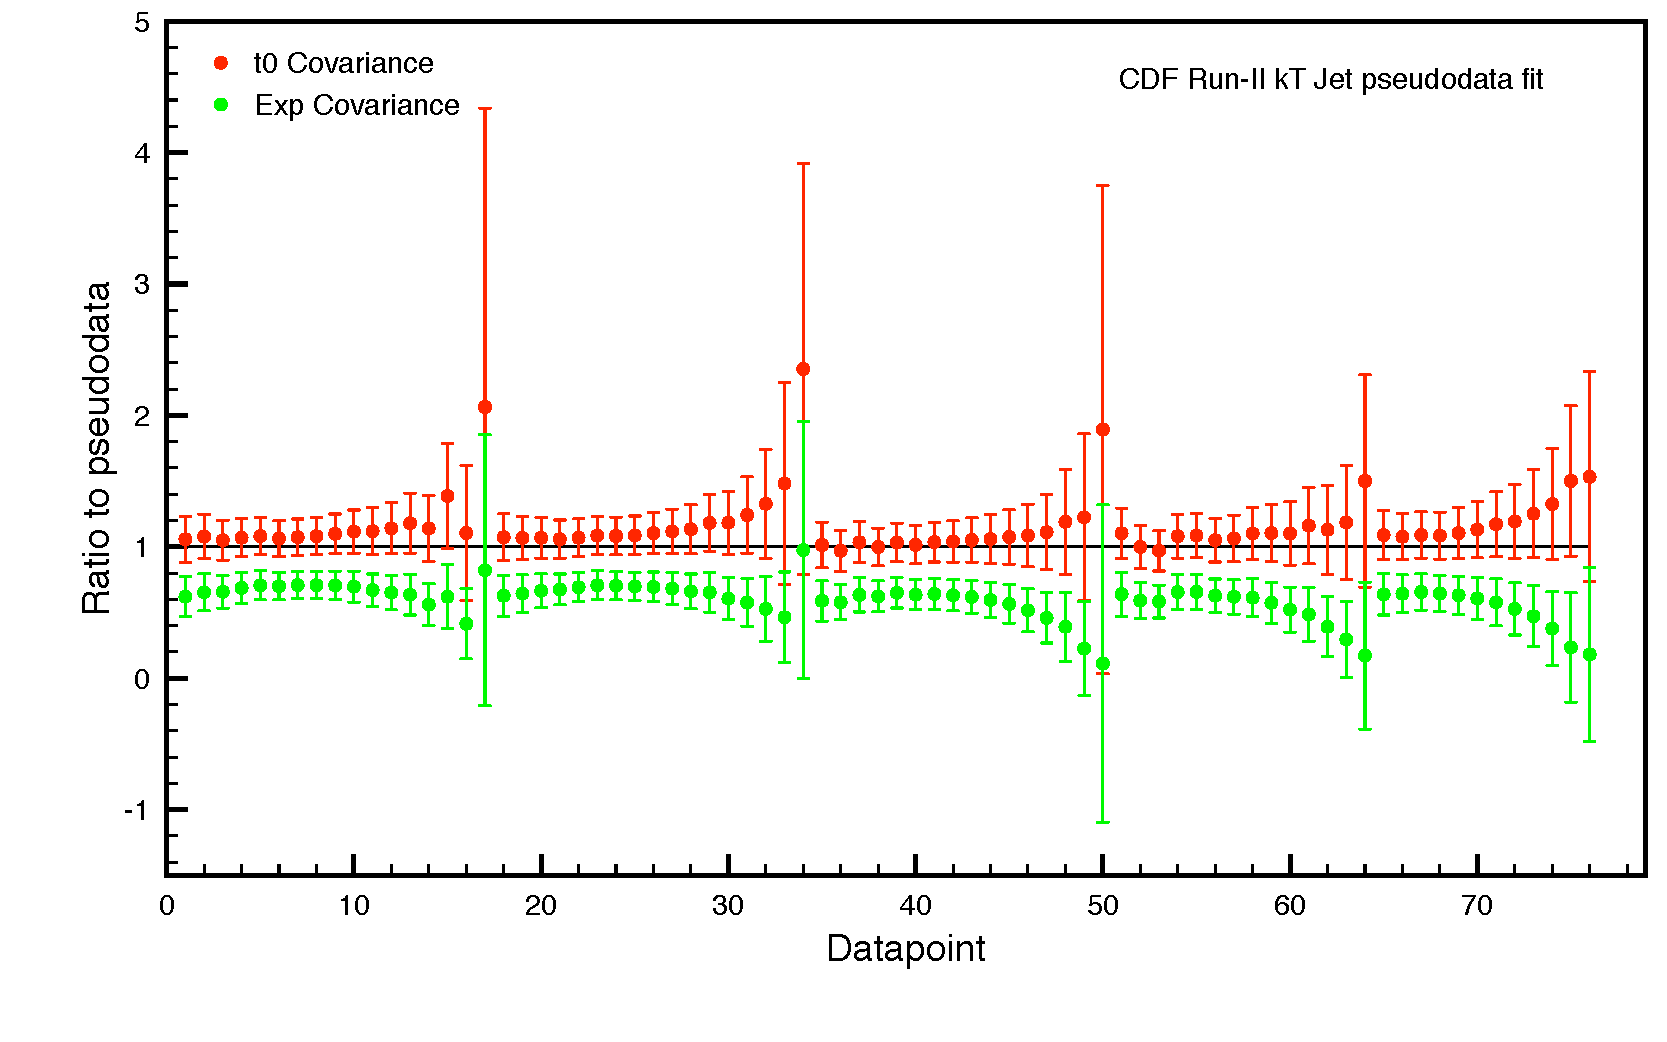
\includegraphics[width=0.8\textwidth]{3-PDFdet/figs/t0plot.pdf}
\caption[Demonstration of d'Agostini bias in a fit to pseudodata generated according to the kinematics of CDF inclusive jet data]{Demonstration of d'Agostini bias in a fit to pseudodata generated according to the kinematics of CDF inclusive jet data. Fit results are shown as a ratio to the `true' value used to generate the pseudodata. The fit performed with the experimental definition of the covariance matrix results in predictions shifted systematically downwards with respect to the underlying law. The predictions from the fit using a $t_0$ covariance matrix do not suffer from such a bias.}
\label{fig:expbias}
\end{figure}

\subsubsection{Minimisation}
With a figure of merit constructed, the PDF determination now becomes a problem of varying the free parameters in the PDF basis to minimise said measure. Even for those groups utilising a fixed parametrisation, performing a minimisation of the global $\chi^2$ for a large, $n\sim\mathcal{O}(1000)$ dataset with a fairly large number of free parameters (approximately $50$ in the MSTW analysis once normalisation uncertainties are added as free parameters) is a challenging numerical task. For performing the minimisation, the MINUIT~\cite{MINUIT} package is a common choice, although other function minimisation methods are applied such as the Levenberg-Marquardt~\cite{levenberg,marquardt} method as used in the MSTW fits.

In the NNPDF case the minimisation is complicated by the very large number of parameters and highly nonlocal behaviour in the error function, making conventional methods of minimisation difficult. These difficulties are overcome in the NNPDF methodology by the use of \emph{genetic algorithms}, which are particularly efficient at exploring large parameter spaces. The implementation of the genetic algorithm is discussed in detail in Refs.~\cite{Ball:2010de,DelDebbio:2007ee}.

In addition to the basic difficulty of minimisation in a large parameter space, there is a further issue that arises when considering the fitting of a function with a great deal of redundant flexibility. Because of the flexibility of the parametrisation, it is possible that training the neural networks so that each reaches the global minimum in the error function actually results in the networks fitting to statistical noise. This effect is known as \emph{overlearning} and is a problem often encountered in the training of large neural networks~\cite{bishopnn,nnoverlearn}. In previous NNPDF determinations, the widely used \emph{cross-validation} technique~\cite{Ball:2010de,bishopnn} was employed in order to identify when overlearning occurred. 

In this method the experimental data set is split into two separate sets. The first, a fitting set which is used for the minimisation of the error function, and a second validation set which is not used directly in the fitting procedure. For each iteration in the genetic algorithm minimisation the error function is computed between the neural network predictions and both data sets. In the early stages of the training both error functions should decrease. However in the latter stages of the training where statistical noise begins to become an important contribution, the goodness-of-fit calculated to the fitting data set may continue to decrease while the same value calculated to the validation set has stopped decreasing or even begun to increase. This is a clear signal of overlearning, where fitting to statistical noise in the fitting set means that the fit to the validation set is no longer improving. At this stage the training of the neural networks is stopped. A typical signal of overlearning in a cross-validated fit can be seen in Figure~\ref{fig:crossval} which compares the fit quality for both the training and validated sets over a number of fit iterations.

\begin{figure}[ht]
\centering
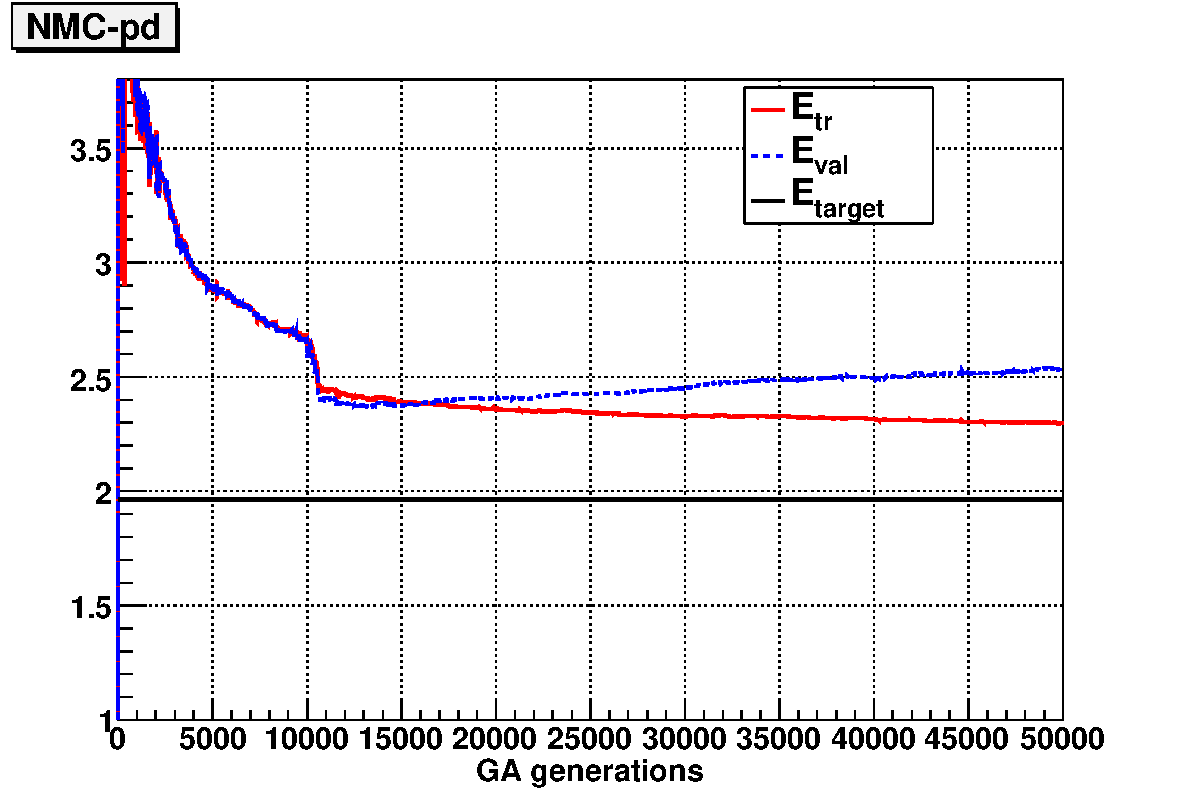
\includegraphics[scale=0.5]{3-PDFdet/figs/chi2ite-1004-NMC-pd.pdf}
\caption[Demonstration of overlearning in the cross-validation of a neural network fit]{A typical signal of overlearning in a neural network fit. E$_{\mathrm{tr}}$ and E$_{\mathrm{val}}$ represent the training and validation figures of merit respectively. As the number of genetic algorithm generations proceeds, eventually the network begins to fit statistical noise in the training set and the validation fit quality begins to decrease. Figure from~\cite{Ball:2010de}.}
\label{fig:crossval}
\end{figure}

\subsection{Error propagation}
\label{sec:errors}
In order to undertake precision QCD studies, some estimate of the uncertainty on PDFs is required for a meaningful interpretation of the measured observables. The need for PDF sets with quantified uncertainties has been long recognised, and all modern determinations provide sets with at least experimental uncertainty estimation. While performing a comprehensive quantification of the theoretical uncertainty in a PDF fit is challenging, many methods have been developed in order to propagate the uncertainty from the dataset to the fitted PDFs. Ideally, one would like to determine a representation of the probability distribution in the whole functional space. That is given a dataset ${d}$, we would like to find the probability of a certain PDF candidate $f$ such that our fitted PDF central value is given by
\be \left<f\right>\left(x\right) = \int \mathcal{D}f \;f\left(x\right)  \mathcal{P}\left(f \middle| d \right), \ee
and the uncertainty by
\be \mathrm{Var}\left[f\right]\left(x\right) = \int \mathcal{D} f \; \left[ f\left(x\right) - \left<f\right>\left(x\right) \right]^2   \mathcal{P}\left(f \middle| d \right). \ee
The probability distribution for an observable $\mathcal{O}$ is then simply $\mathcal{O}\left[f\right]\mathcal{P}\left(f \middle| d \right)$, in terms of which an observable's central
value and PDF uncertainty can be calculated by
\be \left<O\right> = \int \mathcal{D}f \; \mathcal{O}\left[f\right]  \mathcal{P}\left(f \middle| d \right), \ee
\be \mathrm{Var}\left[\mathcal{O}\right] =  \int \mathcal{D}f \; \left(\mathcal{O}\left[f\right] - \left<\mathcal{O}\right> \right)^2 \;\mathcal{P}\left(f \middle| d \right). \ee
The probability distribution $\mathcal{P}\left(f \middle| d \right)$ is however a difficult quantity to determine. In this section we shall examine a number of the methods used in the literature to provide an estimate of PDF uncertainties.
\subsubsection{The Hessian method}
The Hessian method is the most widely used method of uncertainty determination in PDFs. In essence, the method involves examining how the fit quality $\chi^2$ varies when the $n$ fit parameters $a$ are perturbed about the values which minimise the $\chi^2$, here denoted by $a^\mathrm{min}$. A tolerance in the $\chi^2$ variation is then chosen, and the error on an observable is determined geometrically from observables calculated with parameters perturbed by the selected tolerance. To examine this quantitatively, we first define the difference in $\chi^2$ from the minimum value
\be \Delta\chi^2(a) \equiv \chi^2(a) - \chi^2(a^\mathrm{min}) = \sum^n_{i,j=1}H_{ij}(a_i-a_i^\mathrm{min})(a_j - a_j^\mathrm{min}), \ee
where the $a_i$ represent the $i$th component of the parameter set $a$ (and likewise, for the minimised set $a^\mathrm{min}$). Here we assume that the variation around the $\chi^2$ minimum is approximately quadratic. The Hessian matrix $H$ has values determined by
\be H_{ij} = \frac{1}{2}  \frac{ \partial^2 \chi^2(a) }{\partial a_i\partial a_j}\bigg|_{\mathrm{min}},  \ee
where the \emph{min} subscript refers to the parameters obtained at the $\chi^2$ minimum Early Hessian uncertainty estimates~\cite{Adloff:2000qk,Alekhin:2002fv} were based upon the standard formula for linear error propagation
\be (\Delta F)^2 = T^2\sum^n_{i,j=1}\frac{\partial F}{\partial a_i}C_{ij}\frac{\partial F}{\partial a_j}, \ee
where $T^2=\Delta\chi^2$ is the tolerance in $\chi^2$ variation and $C=H^{-1}$ is the inverse Hessian matrix. This procedure is however a little inconvenient due to the requirement of the partial derivatives of the observable with respect to the fit parameters. There are also numerical issues relating to this method which give rise to peculiar uncertainty estimates~\cite{DeRoeck:2011na}.  In order to overcome these issues the geometrical method outlined above was developed by the CTEQ collaboration~\cite{Pumplin:2000vx,Pumplin:2001ct}.

For this method it is convenient to work in a rescaled orthogonal eigenbasis for the covariance matrix. The orthonormal eigenbasis is defined in the usual way

\be H v_i = \lambda_i v_i, \ee
and the rescaled eigenbasis is defined as $e_{i}=1/\sqrt{\lambda_i} v_{i}$. The difference between a parameter set $a$ and $a^\mathrm{min}$ can now be expanded as
\be a_i-a_i^\mathrm{min} = \sum^n_{k=1}e_{ik}z_k, \ee
where $e_{ik}$ is the $i$th component of the $k$th rescaled eigenvector, and the $z_k$ are the coefficients for the expansion of the parameter difference onto the rescaled eigenbasis.  Therefore the expression for $\Delta\chi^2$ reduces to
\be\Delta\chi^2(a) = \sum_{k=1}^n z_k^2 \quad\quad \mathrm{or,}\quad\quad \chi^2(a) = \chi^2(a^\mathrm{min}) + \sum^n_{k=1}z_k^2.\ee
This defines a hypersphere in the parameter space of radius $\Delta\chi^2$ centred around $a^\mathrm{min}$, which corresponds to the variation in the parameters that is consistent with the tolerance $T=\sqrt{\Delta\chi^2}$ in the quadratic approximation. It is now possible to construct an ensemble of $2n$ PDF sets corresponding to the fits on the boundaries of the volume. A PDF set $S^\pm_k$ therefore has the parameter set
\be a_i(S_k^\pm) = a_i^\mathrm{min} \pm te^{ik},\ee
i.e. each parameter is perturbed by $t$ in the direction of the $e_{k}$ eigenvector. In the quadratic approximation $t=T$, when the approximation breaks down $t$ can be determined by an iterative procedure to obtain the desired $\Delta\chi^2$. The error on an observable $F$ is then given simply by Pythagoras' theorem on the hypersphere
\be(\Delta F)^2=\frac{1}{2}\sum_i^n(F(S^+_i)-F(S^-_i))^2.\ee 

In this procedure there is something of an ambiguity in the determination of the tolerance (and hence, the volume of the sphere in parameter space). Ideally the difference in $\chi^2$ values should be exactly one for a confidence level of one-sigma\footnote{It should be noted that this is only the case when, either the data errors are uncorrelated, or when the correlations are included in the definition of the global goodness-of-fit $\chi^2$\cite{Stump:2001gu}}. In the case of PDF fits, this tolerance often leads to uncertainties far lower than expected. In practice, the CTEQ group uses a value of $\Delta \chi^2\sim 100$ and MSTW uses a value $\sim50$. The more recent MSTW PDF sets have uncertainties calculated with a dynamically determined tolerance. More specialised fits such as ABM11 or the HERAPDF series,  based upon relatively restrictive datasets may use the standard tolerance of $\Delta\chi^2=1$. Their use of a more restrictive dataset perhaps leading to fewer conflicts between experimental datasets that could require a more flexible tolerance.

The uncertainties produced via the Hessian procedure are difficult to analyse in a statistical sense due to the (occasional) inflation of the $\Delta\chi^2$ and the approximations made in the procedure. It is therefore difficult to find a representation in the Hessian approach of the full probability distribution $\mathcal{P}\left(f \middle| d \right)$. Furthermore the uncertainty in the choice of functional form, or estimation of parametrisation bias, is not typically take account of. The HERAPDF family of fits however do attempt to estimate this uncertainty by performing a series of fits with slightly modified parametrisations.

\subsubsection{Lagrange multiplier method}
Another method of error propagation that has been explored is the Lagrange multiplier method. The method has the advantage of not assuming that the $\chi^2$ function is quadratic around the global minimum. We shall briefly discuss the method applied to the PDF error determination as suggested by Pumplin~\cite{Pumplin:2000vx} and Stump~\cite{Stump:2001gu}. A description of the process can also be found in~\cite{DeRoeck:2011na,Martin:2009iq}.

Firstly, a general global fit is performed to the data as described above. This yields a set of parameters ${a^\mathrm{min}}$ which minimise the $\chi^2$ measure. Using these parameters we calculate
the best fit prediction for the observable in question $F(a^\mathrm{min})$. A new PDF fit can now be performed, where instead of minimising the $\chi^2$ the following function is minimised
\be \Psi= \chi^2(a) + \lambda (F(a)-F(a^\mathrm{min}))\ee
i.e. we introduce the observable $F$ as a parameter in the fitting procedure and constrain the fit so that the minimal $\Psi$ occurs when $F(a)=F(a^\mathrm{min})$. The value $\lambda$ in this function is the Lagrange multiplier. The fit above is performed for many values of $\lambda$, each time leading to a parameter set that depends on that particular value of $\lambda$, this parameter set will be denoted $a_\lambda$. Using these parameters, we now calculate values for $\chi^2(a_\lambda )$ and $\mathcal{O}(a_\lambda )$.

At this stage we now have a set of values for $\chi^2(a_\lambda)$ and $\mathcal{O}(a_\lambda)$ over a large range of $\lambda$ values. This allows a determination of the relationship between the goodness-of-fit and the prediction for $F$ via the parameter $\lambda$. We obtain an approximate function $\chi^2(F)$ over a range of observable values, with a minimum at $F=F(a^\mathrm{min})$ i.e $\lambda=0$ and $a_\lambda=a^\mathrm{min}$. Also we have a set of the $a$ parameters for every point on the curve which are optimised for the best fit to the observable $F$. This means that we have a set of fully optimised parameters for any arbitrary confidence level determined by the $\Delta\chi^2$ that we select as a tolerance. Uncertainties for the PDFs can therefore be given in a way that utilises the whole of the $a$ parameter space, rather than just perturbing around the global minimum as in the Hessian approach.

Of course, the disadvantage of this method is that the PDF uncertainties must be calculated for each observable in a rather computationally intensive process. The errors are naturally optimised for the particular observable, but the process is inconvenient for a PDF end-user, and so it is not widely-used in error determination. In this sense the Lagrange multiplier approach suggests a method of estimating $\mathcal{P}\left(\mathcal{O} \middle| a \right)$, or the probability density of an observable in the space of parameters. The Lagrange multiplier method also relies on the same somewhat arbitrary choice of tolerance in $\chi^2$ as the Hessian method. The method has however been applied as a cross-check to the Hessian results~\cite{Pumplin:2000vx,Martin:2002aw}.

\subsubsection{Monte Carlo method}
Another quite distinct method of PDF uncertainty determination is the Monte Carlo method, first suggested by Giele and Keller~\cite{Giele:1998gw,Giele:2001mr} where a Monte Carlo procedure in the space of fit parameters was outlined. The NNPDF collaboration uses a similar method in all of its fits, although with the Monte Carlo performed in the space of experimental data. The method is designed to faithfully represent the uncertainties present in the initial data, and to propagate the errors in a way that does not assume anything of the nature of the error propagation. The Monte Carlo approach was also analysed and compared to the results of a Hessian fit by the MSTW group in~\cite{Watt:2012tq}.

In the Monte Carlo procedure an ensemble of $N_{\text{rep}}$ artificial data replicas is produced for every data point in the fit, generated according to the probability distribution of the initial data. Typically this distribution is multi-Gaussian with central values and variances provided by experimental results, but any probability distribution may be used if required. If we use $F_{p}^{(\mathrm{art})(k)}$ to represent a single element $k$ of the pseudo-data sample (the \emph{art} superscript designates the data as an artificial sample) of the observable $F$ at the kinematical point $\left\{ x_p,Q^2_p \right\} $. Then we can generate such a pseudo-data element as in~\cite{Ball:2008by} by
\be F_{p}^{(\mathrm{art})(k)}=S_{p,N}^{(k)}F_{p}^{(exp)}\left( 1 + \sum_{l=1}^{N_c}r_{p,l}^{(k)}\sigma_{p,l} + r_{p}^{(k)}\sigma_{p,s}\right),\ee
where the $r$ are independent Gaussian random numbers centred upon the experimental central value. The $\sigma_{p,s}$ term contains the uncorrelated systematic uncertainties and the statistical uncertainty added in quadrature. The $\sigma_{p,l}$ are the correlated errors for the data provided by experiment. The normalisation of the probability distribution is fixed by the term $S_{p,N}$. Provided a large enough quantity of these artificial replicas ($N_{\mathrm{rep}}$) is generated, this form of the generating distribution for the Monte Carlo ensemble reproduces all of the statistical qualities of the original experimental data. In Ref.~\cite{Ball:2010de} it is demonstrated that $N_{\mathrm{rep}}=1000$ is sufficient to reproduce the experimental central values and variances to an accuracy of better than one percent.

Now that a good Monte Carlo sample of the experimental data is available, instead of performing just the one fit to the data, $N_{\mathrm{rep}}$ independent fits are performed, one for each of the data replicas. At the end of the fitting procedure we obtain an ensemble of $N_{\mathrm{rep}}$ equally probable PDFs which reliably describe the probability distribution of the PDFs based upon the original experimental uncertainties. The central values and uncertainties of an observable can be simply obtained by computing the average and the variance over the ensemble of PDFs.
\be \left< F\right> = \frac{1}{N_{\mathrm{rep}}}\sum_i^{N_{\mathrm{rep}}} F^{(k)}, \label{eq:MCCV}\ee
 \be \sigma^2[F] = \frac{1}{N_{\mathrm{rep}}-1} \sum_{i=1}^{N_{\mathrm{rep}}} (F^{(k)} - \left< F\right>)^2, \label{eq:MCVAR}\ee
 where $F^{(k)}$ denotes the observable $F$ computed using PDF replica $k$.

The Monte Carlo method therefore propagates the errors from the experimental data through to the PDFs in a natural way, without the need for a linear propagation of errors assumption, or the need for an inflated tolerance in the $\chi^2$ distribution. Figure \ref{fig:mcerror} demonstrates a Monte Carlo ensemble of PDF replicas for the gluon distribution.

\begin{figure}[ht]
\centering
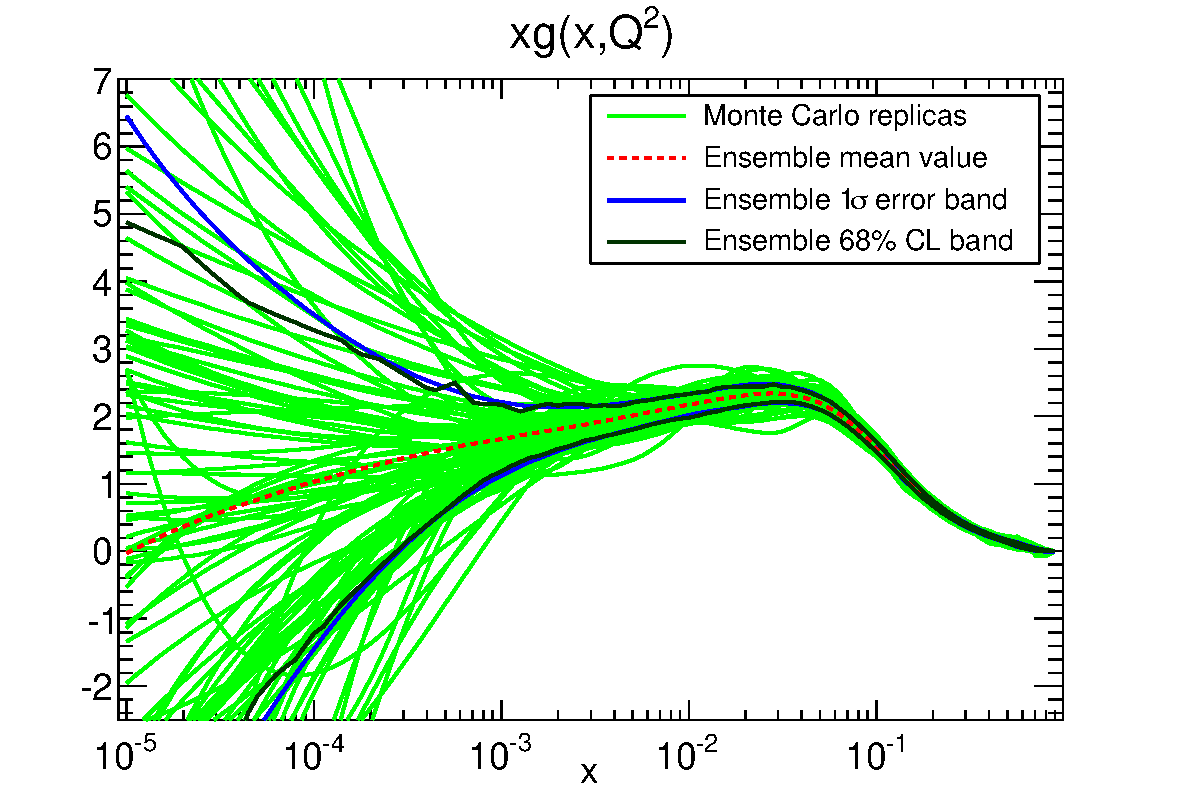
\includegraphics[width=0.48\textwidth]{3-PDFdet/figs/pdf_xg_log_rep.pdf}
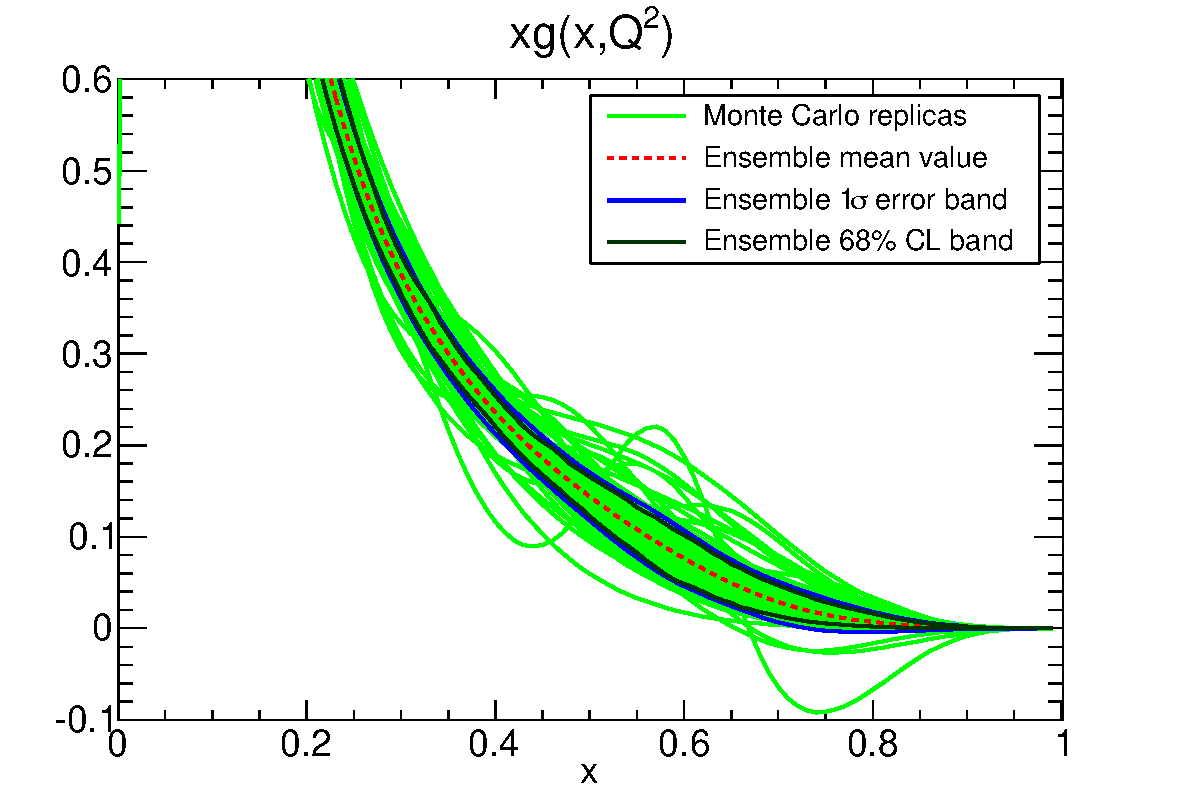
\includegraphics[width=0.48\textwidth]{3-PDFdet/figs/pdf_xg_rep.pdf}
\caption[A Monte Carlo representation of the gluon PDF probability distribution]{A Monte Carlo representation of the gluon PDF probability distribution. Individual PDF replicas are shown as green lines, and the ensemble average, standard deviation and 68\% confidence level are shown.}
\label{fig:mcerror}
\end{figure}

%
%In the NNPDF approach the method has another benefit. Considering again the method of cross-validation used to prevent overfitting in the neural network parametrisation. At first glance, it would seem that separating the data sets into a fitting and validation set means that not all of the data is directly used in a fit. However, as the selection of data points for each set is done at randomly on a replica, by replica basis, for a large enough $N_{\mathrm{rep}}$ the whole data set is used for fitting across the ensemble.  The use of an ensemble of replicas additionally helps with estimating the functional uncertainty present when determining a function from a finite set of data points. 
%
%\subsection{Sources of theoretical uncertainty}
%
%
%Maybe have here a short summary of all the sources of theoretical uncertainty, and how they may be taken into account?
%alphas, GM scheme, deuteron/nuclear corrections, fragmentation in prompt $\gamma$, NP uncertainties e.g hadronisation/pileup.

\section{Status of PDF determination before the LHC}
In preparation for the application of parton distributions at the LHC, extensive studies were performed in order to benchmark and understand areas of agreement and discrepancy across fitting collaborations~\cite{Watt:2011kp,Dittmar:2009ii}. While agreement had generally improved as the level of sophistication applied in parton fits increased, there were still notable regions where PDF fits from the widest datasets remained in disagreement at levels greater than their quoted uncertainties. Figure \ref{fig:pdflumidiff} illustrates the situation for two important PDF luminosities before the LHC. These discrepancies extended not only to so far unmeasured quantities such as Higgs production cross sections, but also to PDF standard candle observables such as $W$ boson production (c.f. Figure \ref{fig:standardcandleerror}).

\begin{figure}[t]
\centering
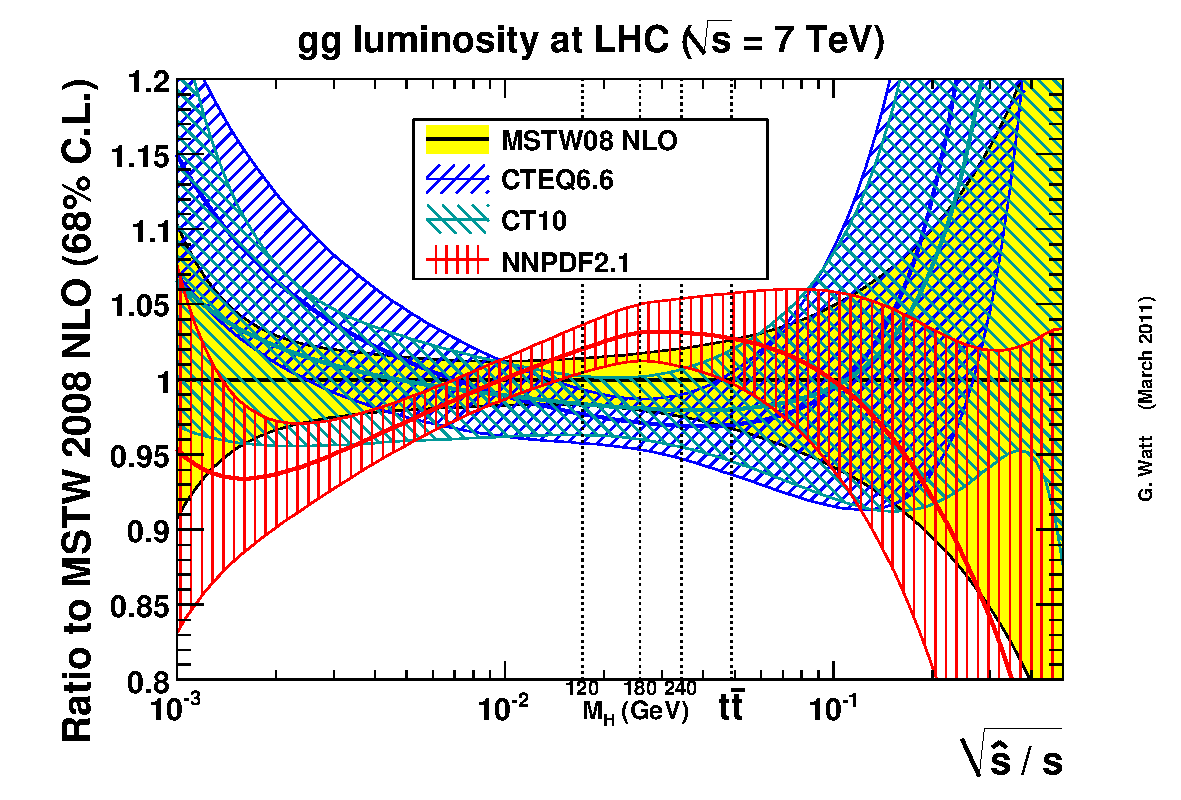
\includegraphics[width=0.48\textwidth]{3-PDFdet/figs/ratiogglumi1_68cl.pdf}
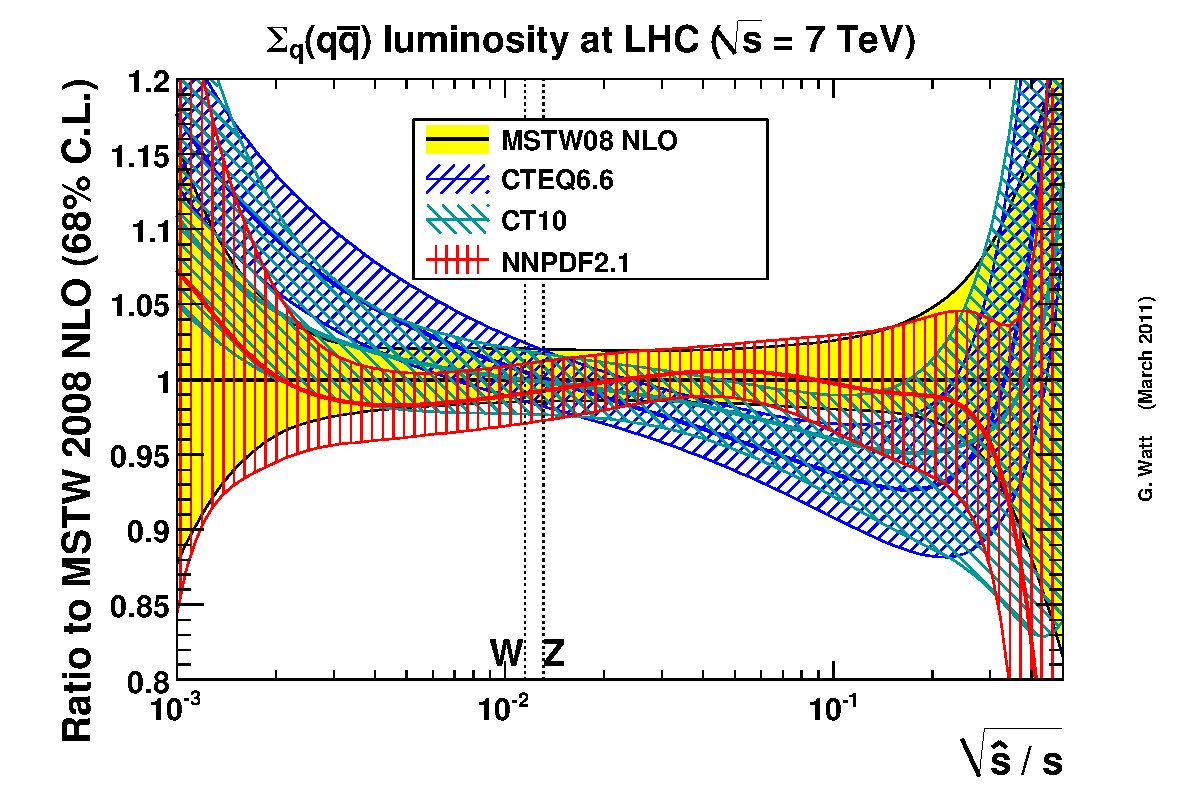
\includegraphics[width=0.48\textwidth]{3-PDFdet/figs/ratioqqbarlumi1_68cl.pdf}
\caption[Luminosities for $gg$ and $q\bar{q}$ PDF combinations at the $7$ TeV LHC]{Luminosities for $gg$ (left) and $q\bar{q}$ (right) PDF combinations at the $7$ TeV LHC. Figure from~\cite{Watt:2011kp}.}
\label{fig:pdflumidiff}
\end{figure}


\begin{figure}[ht]
\centering
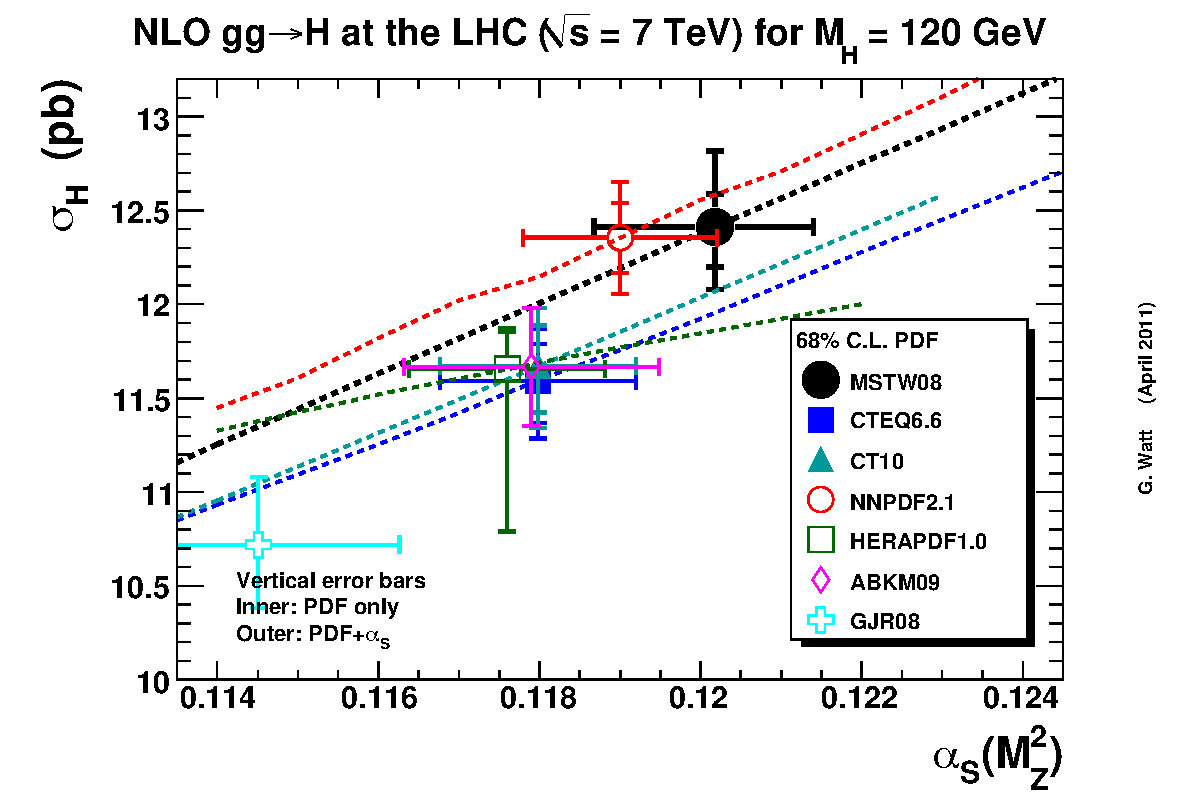
\includegraphics[width=0.48\textwidth]{3-PDFdet/figs/ggH120GeVLHC7TeVnlo68cl.pdf}
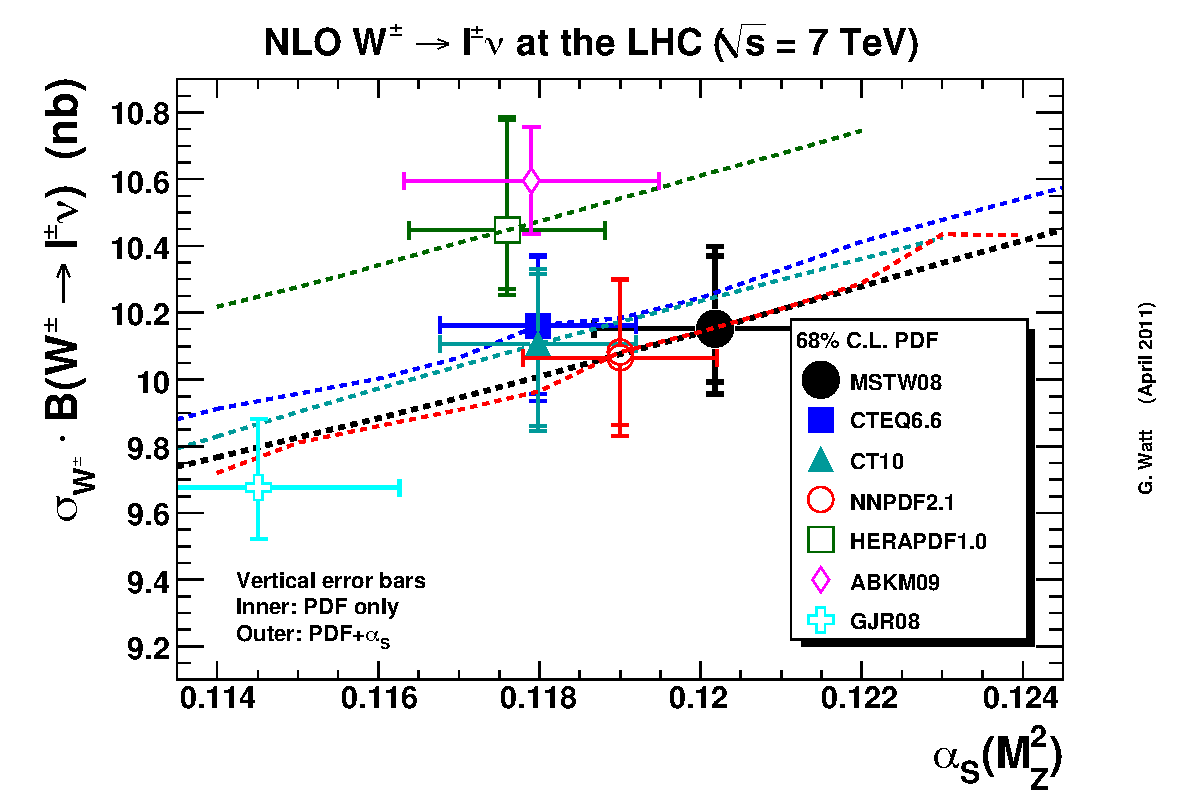
\includegraphics[width=0.48\textwidth]{3-PDFdet/figs/wpmLHC7TeVnlo68cl.pdf}
\caption[Predictions for example LHC processes based upon a number of PDF determinations]{Predictions for LHC processes based upon a number of PDF determinations. Left figure: cross section for Higgs production in gluon fusion. Right figure: cross section for the production of $W$ bosons. Figure from~\cite{Watt:2011kp}.}
\label{fig:standardcandleerror}
\end{figure}
The Les Houches benchmark exercise~\cite{Dittmar:2009ii} helped to elucidate the methodological source of many of these differences by testing fits from various methodologies to a standard dataset.

Many of the observed discrepancies arise due to differences in the theoretical description of data, with the choice of flavour number scheme providing the largest differences. Dataset choice and methodological choices introducing significant differences also. These differences led to the conservative PDF4LHC recommendation for observables to be calculated as the central contour of the CTEQ-MSTW-NNPDF uncertainty envelope. Despite the differences, for the LHC Run-I the range of available sets allowed for experimental collaborations to effectively explore the differences in the resulting predictions.

While providing accurate determinations for use at the LHC has been the primary concern in the years leading up to the LHC's first operation, there was substantial interest in the potential of the LHC to provide constraints upon PDFs and potentially provide discriminating power between sets. Data from the LHC provides the best opportunity for distinguishing the most effective approaches both theoretically and methodologically. Additionally LHC data provides particularly valuable input in the field of collider-only determinations, which aim to provide a cleaner description of data by avoiding the inclusion of nuclear-corrected and low energy data. The inclusion of a large LHC dataset into PDF fits is however a challenging problem, and one which has inspired a great deal of progress in the efficient calculation of collider observables. The remainder of this work will therefore deal with the both the technical inclusion of LHC data into parton distribution fits and the subsequent phenomenological results.

